% ######################################################################
%
% 			PREAMBULE
%
% ######################################################################

% -------------------------------------------------------
% Ce document est un raport. dizaine de pages / plusieurs sections
% -------------------------------------------------------
\documentclass[a4paper,12pt]{report}

% -------------------------------------------------------
% Utiliser latin1 pour les accents
% ne pas utiliser utf8 et Latex n'aime pas utf8 ET latin1
%\usepackage[utf8]{inputenc}
% -------------------------------------------------------
\usepackage[utf8]{inputenc}

% Vu dans un forum : utiliser plutôt frenchb, french est obsolete
\usepackage[T1]{fontenc}
\usepackage[english,frenchb]{babel}

\usepackage{amsmath}
\usepackage{amssymb}
\usepackage{amsfonts}
\usepackage{array}
\usepackage{booktabs}
\usepackage{diagbox} % barre oblique pour les cellule à 2 entrées
\usepackage[pdftex]{graphicx}
\usepackage{hhline}
\usepackage{hyperref}
\usepackage{lmodern}
\usepackage{multicol}
\usepackage{subcaption}
\usepackage{supertabular}
\usepackage{textcomp}
\usepackage{xcolor}
\usepackage{xspace}

% -------------------------------------------------------
% Théorèmes
% -------------------------------------------------------
\usepackage{amsthm}
\theoremstyle{plain}				% Choix du style
\newtheorem{theoreme}{Théorème}	% Définition de l'environnement 1
\newtheorem{example}{Exemple}
\theoremstyle{definition}				% Choix du style
\newtheorem{definition}{Définition} %[section]	% Définition de l'environnement définition

% -------------------------------------------------------
% Pour les ALGORITHMES
% linesnumbered	: les lignes sont numérotées
% ruled			: Le caption est en haut et bordé de lignes horizontale
% vlined		: Regroupement des bloc d'instructions par ligne verticales
% -------------------------------------------------------
\usepackage[linesnumbered, ruled, vlined, french]{algorithm2e}

% Commandes en français:
\SetKwInput{KwRes}{R\'esultat}%
\SetKw{WEntree}{\textcolor{red}{Entrée}}
\SetKw{WEntrees}{\textcolor{red}{Entrées}}
\SetKw{WSaisir}{Saisir}
\SetKw{WInitialisation}{\textcolor{red}{Initialisation}}
\SetKw{WTraitement}{\textcolor{red}{Traitement}}
\SetKw{WAssigne}{\textcolor{blue}{prend la valeur}}
\SetKw{WSortie}{\textcolor{red}{Sortie}}
\SetKw{WSorties}{\textcolor{red}{Sorties}}
%
\SetKwIF{Si}{SinonSi}{Sinon}{Si}{alors}{sinon si}{sinon}{fin si}
\SetKwFor{Tq}{Tant que}{faire}{fin tantque}
\SetKwFor{Pour}{Pour}{faire}{fin pour}
\SetKw{WAfficher}{Afficher}
\SetKwRepeat{Repeter}{répéter}{jusqu'à}%
%
\SetKw{Return}{\textcolor{red}{Renvoyer}}%
%
\SetKwProg{Init}{init}{}{}
% mettre les commentaire des algos en bleu

% -------------------------------------------------------
% Information PDF généré
% -------------------------------------------------------
\hypersetup{pdftex, colorlinks=true, linkcolor=blue, citecolor=blue, filecolor=blue, urlcolor=blue, pdftitle=, pdfauthor=Florian Colas, pdfsubject=, pdfkeywords=}

% -------------------------------------------------------
% MACRO
% -------------------------------------------------------
% Pm||Cmax
\newcommand\problemGrahamPm{$P_m||C_{\max}$\xspace}
% P2||Cmax
\newcommand\problemGrahamPII{$P_2||C_{\max}$\xspace}	%apparemment ne supporte pas les chiffres.
% P||Cmax
\newcommand\problemGrahamP{$P||C_{\max}$\xspace}

% -------------------------------------------------------
% Ajout L. Philippe
% Utilisation des Todo inline en macro --> tdi
% -------------------------------------------------------
\usepackage{todonotes}
\newcommand{\tdi}[1]{\todo[inline]{{#1}}{}}
\newcommand{\lp}[1]{\todo[author=LP,color=yellow,inline]{#1}}
\newcommand{\lcc}[1]{\todo[author=LCC,color=green,inline]{#1}}
\newcommand{\fco}[1]{\todo[author=FCO,color=blue,inline]{#1}}
\newcommand{\jb}[1]{\todo[author=JB,color=orange,inline]{#1}}

% -------------------------------------------------------
% Information générales
% Utilisé par \maketitle
% -------------------------------------------------------
\title{Historique des travaux autour du problème $P||C_{\max}$}
\author{Florian Colas}
% \date{2020-05-01}
\date{\today}

% -------------------------------------------------------
% POUR PAGE DE GARDE
% -------------------------------------------------------
%\setlength{\parindent}{0cm}
%\setlength{\parskip}{1ex plus 0.5ex minus 0.2ex}
%\newcommand{\hsp}{\hspace{20pt}}
%\newcommand{\HRule}{\rule{\linewidth}{0.5mm}}
%\usepackage{titling}

% ######################################################################
%
% 			SOUVENT UTILISES
%
% ######################################################################
% Pm||Cmax 				: \problemGrahamP
% P2||Cmax 				: P\textsubscript{2}{\textbar}{\textbar}C\textsubscript{max}
% P||Cmax 				: P{\textbar}{\textbar}C\textsubscript{max}
%
% Appostrophes 			: '
%
% en italique car latin : \textit{et al.}
%
% entourer un résultat
%	\begin{center}
%	\fbox{\begin{minipage}{\linewidth}
%	bla blabla
%	\end{minipage}}
%	\end{center}


% ######################################################################
%
% 				DOCUMENT
%
% ######################################################################

\begin{document}

% =======================================================
% Page de garde
% Utilise Information générales
% Ecrit le titre + auteur + date
% =======================================================
%\maketitle
\begin{titlepage}
%-------------------------------------------
% LOGOS / 
%-------------------------------------------
\begin{center}

\includegraphics[width=3cm]{logo_CTU_2018.png}
\hfill
\parbox{.5\linewidth}{%
	\centering
	Universit\'e de Franche-Comté	\par
	Master 2 I2A	année 2020 / 2021 \par
	Florian Colas / 21512327
	\vspace{.05\textheight}
	\vspace{.05\textheight}
}
\hfill

\includegraphics[width=3cm]{logo_UFC.png}

%-------------------------------------------
% MODULE
%-------------------------------------------
\vspace{.05\textheight}
{\LARGE\scshape Module EPR\par}

%-------------------------------------------
% TITRE DE L'ETUDE
%-------------------------------------------
\vspace{.05\textheight}
\vspace{.05\textheight}
\vspace{.05\textheight}
{\Huge\bfseries Historique des travaux autour du problème \problemGrahamP \par}

%-------------------------------------------
% SUPERVISEURS
%-------------------------------------------
\vspace{.05\textheight}
\vspace{.05\textheight}
\vspace{.05\textheight}
Encadrants
\vspace{.05\textheight}
\begin{tabular}{llll}
Laurent Philippe & Professeur &  &  	\\
Louis-Claude Canon & Maître de conférence &  &  \\
Julien Bernard & Maître de conférence &  &  	\\
\end{tabular}
  
\end{center}
\end{titlepage}



% -------------------------------------------------------
% Table des matières
%
% On renomme en Sommaire (document français)
%
% On définit la profondeur de la table des matières
% -1 partie,    0 Chapitre,
% 1 Section,    2 sous sections,  3 sous sous section
% 4 Paragraphe, 5 Sous paragraphe
%
% Les sections sont numérotées 1 2 3
% -------------------------------------------------------
\renewcommand{\thesection}{\arabic{section}}
\renewcommand{\contentsname}{Sommaire}
\setcounter{tocdepth}{3}	% avant 2 pour la table des matières
\setcounter{secnumdepth}{3}	% pour les section sous et sous sous et paragraphes
\tableofcontents

%\lcc{Suggestions, peut-être un peu tardive, sur l'organisation du
%  document.
%  Faire sauter un niveau en sous-section 3.3 (3.3.1 deviendrait une
%  sous-section).
%  Faire sauter un niveau en section 5 (5.1 deviendrait 5 et 5.2 serait
%  un paragraphe de perspectives qui conclurait la section 5).
%  Faire sauter un niveau en sous-section 6.1 (pareil, on conserve le
%  premier paragraphe introductif, on enlève la sous-sous-section
%  6.1.1, et on intègre 6.1.2 en tant que paragraphe d'ouverture).
%  Je mettrais aussi LDM dans la section heuristique.
%  Finalement, je mettrais aussi 6.2 en tant que 7.3 pour le recul
%  général.
%  Ça donnerait (à partir de 3.3): 3.3 Slack; 3.4 LDM; 4 Programmation
%  linéaire; 5 PTAS Dual; 6 Synthèse; 6.1 Comparaisons...; 6.2
%  Recherche...; 6.3 Limites de l'étude, ou quelque chose du genre.
%}
% \fco{Mis d'accord avec Louis --> le faire plus tard car pas le temps}

%\lp{Remarque générale: ajouter un peu de blabla pour rendre moins
%  lapidaire?}

% =======================================================
% 1 INTRODUCTION
% =======================================================
\section{Introduction} \label{sec:introduction}

Qu'ont en commun les lignes de productions industrielles, la gestion
des quais d'expédition, l'organisation de partiels d'une université,
la fabrication d'une maison, la planification des opérations d'un
hôpital, ou l'attribution de tâches à un microprocesseur multi-cœurs?
Chacune de ces activités demande la résolution d'un problème
d'ordonnancement, afin d'optimiser un coût, des priorités, un retard
ou un temps total.

Graham (1935 - 2020) est l'un des pionniers dans l'analyse
mathématique du problème d'ordonnancement, et relève certaines
anomalies \cite{graham1966bounds}: Des tâches dont certaines sont
reliées entre elles par des contraintes, et exécutées en parallèle
seront traitées en moins de temps que si les contraintes sont
supprimées.
D'où l'importance de la planification des tâches.

Le problème \problemGrahamP consiste à planifier des tâches, sur des
machines parallèles, dans le but de minimiser le temps total de
traitement (makespan).
Malgré cette apparente simplicité, le problème est NP-Difficile, de
même que ses problèmes similaires, Bin-packing, et partition de
nombres.
Les algorithmes développés tentent de donner une solution la plus
proche possible de la solution optimale, dans les meilleurs délais.

Ce document tente d’énumérer et de présenter les algorithmes les plus
courants ainsi que les différentes méthodes de résolution utilisées.
Après une présentation du problème (section~\ref{sec:pesentationProbleme}),
nous étudierons, dans un premier temps, diverses heuristiques (section~\ref{sec:heuristiques}),
  plus précisément l'utilisation des ``list scheduling'',
  et des outils de résolution du problème Bin-packing.
Ensuite, nous verrons comment la programmation linéaire
  (section~\ref{sec:programmationLineaire}) peut résoudre le problème,
suivi par l'étude de la définition d'un schéma d'approximation
  en temps polynomial (PTAS) (section~\ref{sec:approximation}).
Le problème de partitionnement de nombres, ainsi que sa
  résolution approchée sera la dernière approche examinée
  (section~\ref{sec:autresApproches}).
Ce document se termine par une synthèse (section~\ref{sec:synthese}).


\section{Présentation du problème} \label{sec:pesentationProbleme}

Le problème d'ordonnancement se pose depuis l'apparition des premières
machines parallèles.
Après un rappel sur le parallélisme, nous verrons les divers problèmes
d'ordonnancement, pour nous concentrer en particulier sur le problème
\problemGrahamP, la problématique que cela pose.


\subsection{Parallélisme} \label{ssec:pesentationProblemeParallelisme}
Le parallélisme est un type d{\textquotesingle}architecture informatique
dans lequel plusieurs processeurs exécutent ou traitent une application
ou un calcul simultanément. Il aide à effectuer de grands calculs en
divisant la charge de travail entre plusieurs processeurs, capables de
communiquer et de coopérer.

% -------------------------------------------------------
% FLYNN 1972
% -------------------------------------------------------
En 1972, Flynn propose une première classification des
architectures parallèles~\cite{5009071}.
Cette taxonomie (table~\ref{table:taxonomyDeFlyn})
repose sur le nombre de flux de données (simple ou
multiple) et le nombre de flux d'instructions (simple ou multiple).
% -------------------------------------------------------
% TABLEAU taxonomie de Flynn
% diagbox permet d'avoir une barre oblique pour les deux entrées
% \backslashbox{Instructions}{Donnée} & Simple & Multiple NE FONCTIONNE PAS
% on cadre à gauche le tableau pour avoir plus de place
% -------------------------------------------------------

\begin{table}
\centering
\begin{tabular}{|p{2.88cm}|p{4.5cm}|p{4.5cm}|}

% --------------------------
% TITRES
% --------------------------
\hline
\diagbox[width=8em]{Instructions}{Données} & Simple & Multiple \\
\hline

% --------------------------
% LIGNE SIMPLE
% --------------------------
Simple

%---------------------------
&
\textbf{SISD}

premiers PC

machine de Von Neumann


microcontrôleurs, \newline Arduino \ldots
%---------------------------
&
\textbf{SIMD}

Machines synchrones

Pipeline	%

Exécution d'une instruction unique sur des données différentes
\\	\hline
% --------------------------
% LIGNE MULTIPLE
% --------------------------
Multiple
%---------------------------
&
\textbf{MISD}

Machines vectorielles

Tableau de processeurs

Exécute plusieurs instructions sur une même donnée
%---------------------------
&
\textbf{MIMD}

Multi processeurs à mémoire distribuée (multi-ordinateurs)

Multi processeurs à mémoire partagée (multi-c{\oe}urs)
%---------------------------
\\
\hline
\end{tabular}
\caption{Taxonomie de Flynn}
\label{table:taxonomyDeFlyn}
\end{table}


% -------------------------------------------------------
% Skilicorn 1988
% -------------------------------------------------------
En 1988, Skilicorn étoffe la taxonomie de Flynn et propose une
classification plus complète \cite{86786}, basée sur l'architecture,
avec 28 taxons
% -------------------------------------------------------
% Dasgupta 1990
% Inutile ici.
% -------------------------------------------------------
% \item en 1990, Dasqupta présente une classification, toujours orientée
% \cite{50273}  3 si pas desactivé

% -------------------------------------------------------
% Duncan 1990
% -------------------------------------------------------
En 1990, Duncan présente une taxonomie de haut niveau \cite{44900}
(figure \ref{fig:TaxonomieHautNiveau}),
reprenant les bases de la classification de Flynn, tout en incluant
les architectures modernes, et celles qui n'ont pas encore été
considérées comme architectures parallèles (e.g les processeurs
vectoriels à chaînes de traitement).

\begin{figure}
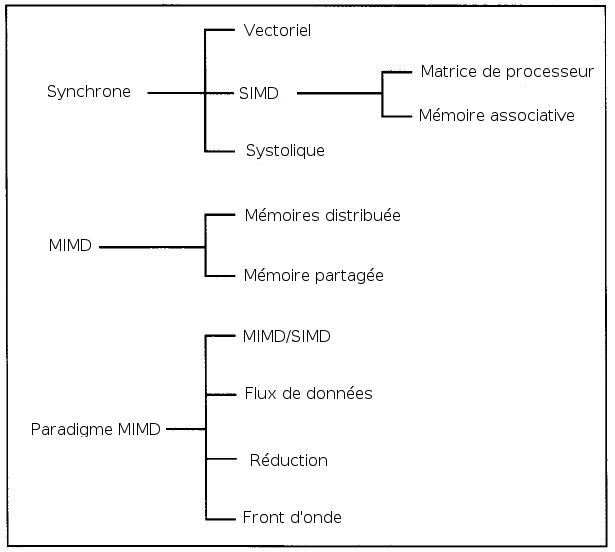
\includegraphics[width=\columnwidth]{Biblio_PCmax_Rendu_Taxonomie_Duncan.jpg}
\caption{Taxonomie de haut niveau de l'architecture de l'informatique parallèle.}
\label{fig:TaxonomieHautNiveau}
\end{figure}

\begin{itemize}
\item Les architecture synchrones.
  Ces architectures coordonnent les opérations concurrentes via une
  horloge globale et un contrôleur de programmes.
  \begin{itemize}
  \item Les processeurs
  vectoriels permettent un traitement parallèle en envoyant
  séquentiellement des éléments vectoriels dans des pipelines d'unités
  de traitements mis en cascades.
  \item Les machines systoliques,
  pulsent le déplacement des données entre mémoire et réseau de
  processeurs, à un rythme soutenu.
  \item Les SIMD, emploient une unité de contrôle centrale, et de
  multiples processeurs.
  On distingue les SIMD à matrice de processeurs, (calibrés pour le
  calcul scientifique à grande échelle, le traitement d'images) où on
  retrouve les GPU, et les SIMD à mémoire associative
  (particulièrement adaptés pour le traitement de bases de données, le
  suivi, la surveillance).
  \end{itemize}
\item Les architectures asynchrones, de type MIMD, emploient plusieurs
  processeurs pour exécuter des flux d'instructions indépendant, en
  utilisant des données locales.
  On distingue, d'une part, les MIMD à mémoire distribuée.
  Les processeurs ont leur propre mémoire, et le partage d'informations
  s'opère uniquement par échanges de messages.
  On rencontre dans ce type d'architecture, les grappes, les MPP
  (Massive Parallel Processing) et les COW (Cluster Of Workstations).
  Et d'autre part les MIMD à mémoire partagées, telles que les
  machines muti-processeurs, ou les processeurs multi-c\oe{}urs. C'est justement dans ce contexte que cette étude se situe.


\item Les architectures mixtes, ou basées sur le paradigme MIMS.
  \begin{itemize}
  \item Les hybrides MIMS/SIMS sont des architectures MIMD pilotées de
  la même façon que les SIMD.
  \item Les architectures à flots de données sont pilotées par les
  dépendances des données elles-mêmes.
  \item Les architectures à réductions sont utilisées pour les langages
  de programmation fonctionnels, dont les expressions sont récursives.
  \item Les architectures Front d'onde (wavefront) sont un mélange des
  architectures à flots de données et des architectures systoliques.
  \end{itemize}

\end{itemize}


Les premières machines parallèles étaient des réseaux
d'ordinateurs, et des machines vectorielles (faiblement
parallèles, très coûteuses), telles que l'IBM 360, les
Cray1.
De nos jours, les super-ordinateurs ont un nombre de c\oe{}urs de
l'ordre de plusieurs millions, et leur performances de calculs
s'expriment
en centaines de petaFLOP. Les 500 super-ordinateurs les plus puissants
sont recensés par le site www.top500.org.
Le Supercomputer Fugaku (Fujitsu), du Centre pour la science
des ordinateurs de RIKEN au Japon (figure \ref{fig:Fugaku}),
vient de détrôner depuis juin 2020 le Summit (IBM)
de l’Oak Ridge National Laboratory aux États-Unis.

\bigskip

\begin{figure}
  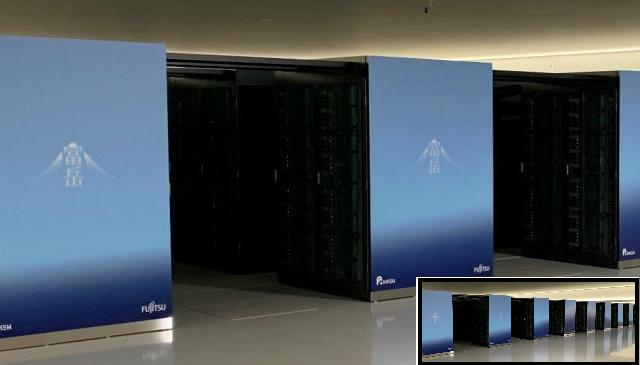
\includegraphics[width=\columnwidth]{Biblio_PCmax_Rendu_Fugaku.jpg}
\caption{Le Supercomputer Fugaku (Fujitsu),
  Il compte 7,630,848 c\oe{}urs basés sur des processeurs ARM A64FX
  48C cadencés à 2.2GHz, 5,087,232 GB de ram, pour une performance de 442 PFLOPS.
  Il fonctionne sous Red Hat Entreprise Linux (RHEL).}
\label{fig:Fugaku}
\end{figure}

On peut définir une machine parallèle comme un ensemble de processeurs
capables de coopérer et de communiquer dans le but de résoudre un
problème plus rapidement.
Les clusters, ou grappes (MIMD à mémoire distribuée), sont
principalement homogènes.
Avec internet, il devient possible d'interconnecter des ordinateurs,
voire des grappes, et de créer ainsi, à l'instar d'un réseau de
distribution d'électricité, un système distribué grande échelle,
appelé grid, ou grille.
Une grille relie des ordinateurs (PC, portable,
Superordinateur, cluster), des systèmes de bases de données
(e.g base du génome humain, atlas astronomique de Strasbourg), et dans
certains cas, des instruments spéciaux
(e.g le radio-télescope d'Arecibo).
Les applications liées aux grilles sont diverses.
On peut citer le web (la première grille), le \emph{Cloud
  computing}, les web-services, les réseaux \emph{peer-to-peer},
l'\emph{internet computing}, comme le projet SETI
(\url{www.boinc-af.org/setihome.html}).
Ce projet consiste à rechercher des preuves possibles de transmissions
radio provenant d'intelligences, autres que terrestres, à l'aide de
données fournies par un radiotélescope.
Le ``serveur'', distribue, une portion d'échantillons radio à traiter
aux clients volontaires (logiciel client installé sur un PC), pour
ensuite recouper les résultats.
En tout, ce sont cinq millions de participants, qui ont accumulé deux
millions d'années de calculs depuis la création du projet en 1999.
Se pose alors le problème de l'attribution des tâches aux postes
clients, un problème d'ordonnancement.


\subsection{Ordonnancement} \label{ssec:pesentationProblemeOrdonnancement}

Sur une machine non parallèle, les tâches sont exécutées
séquentiellement, les unes après les autres.
Certaines tâches, ou jobs peuvent demander plus de temps que d'autres
pour être entièrement traitées.
Lorsque plusieurs ressources (processeurs, machines, cœurs) sont
disponibles, ou que des jobs a exécuter ne sont pas indépendants (même
traités sur un seul processeur), se pose alors, un problème
d'ordonnancement.
Celui-ci consiste à organiser, dans le temps, les jobs à exécuter, en
les affectant à une ressource donnée, de manière à satisfaire un
certain nombre de contraintes, tout en optimisant un ou des objectifs.
L'ordonnancement fait partie de la catégorie des problèmes
d'optimisation combinatoire, et est un champ de la recherche
opérationnelle, très actif depuis plus d'un siècle.

Les problèmes qui s'y rattachent sont très variés.
Premièrement, la nature des machines parallèles doit être considérée.
Celles-ci peuvent être:
\begin{description}
\item[identiques] le même temps de traitement sera nécessaire, d'une
  machine à l'autre;
\item[uniformes] un quotient de vitesse $q_i$ propre à une machine est à
  appliquer pour chaque tâche affectée à cette machine pour déterminer
  le temps de traitement nécessaire;
\item[indépendantes] les temps de traitements des tâches sont ni
  uniformes ni proportionnels d'une machine à l'autre.
\end{description}
Ensuite, des contraintes peuvent affecter les jobs eux-mêmes.
Dans le cas d'un problème préemptif, les tâches peuvent être
interrompues, et reprises ultérieurement.
Il est possible que les jobs soient indépendants, ou au contraire,
être liées par des relations de précédence.
Ces jobs ne sont disponibles qu'à partir d'une certaine date.
Ou encore, être de durée égale, ou tous de durée différente.

Pour finir, l'objectif de
l'ordonnancement est d'optimiser un
critère. Par exemple, minimiser la somme des dates de fin, la somme
des retards, le nombre de tâches en retard, ou simplement, le retard
total. Mais le plus habituel, est de chercher à minimiser le temps
total de traitement de tous les jobs, i.e.\ minimiser le makespan noté $C_{\max}$.


Ces diverses possibilités définissent divers problèmes
d'ordonnancements différents, recensés et classifiés
par Graham \emph{et al.} \cite{graham1979optimization}, qui introduit
la notation trois-champs $\alpha
${\textbar}$\beta ${\textbar}$\gamma $ .

\bigskip

Dans cette classification, le problème \problemGrahamP se définit alors ainsi:

\begin{itemize}

% -------------------------------------------------------
% ALPHA P Type de machines
% -------------------------------------------------------
\item $\alpha = \alpha_1 \alpha_2$, détermine l'environnement machines.
  \begin{itemize}
  \item $\alpha_1 = P$:
  les machines sont parallèles et identiques: un job,
  une tâche prendra le même temps de traitement qu'il soit exécuté sur
  une machine ou une autre.
  \item $\alpha_2$:
  Si $\alpha_2$ est un nombre positif, alors, le nombre de machines ($m$)
  et constant et est égal à $\alpha_2$ (e.g. $P_2$).
  Si $\alpha_2 = \emptyset$ alors le nombre de machines ($m$) est variable.
\end{itemize}
% -------------------------------------------------------
% BETA Contraintes
% -------------------------------------------------------
\item
  $\beta$  détermine les caractéristiques des jobs, ou des
  tâches. Ici $\beta = \emptyset$ (est vide), ce qui signifie que la préemption
  n'est pas autorisée (les jobs doivent être exécutés d'une traite,
  sans interruption ni coupure) et qu'il n'y a pas de relation entre
  les jobs (ils sont indépendants).

% -------------------------------------------------------
% GIMEL Optimisation
% -------------------------------------------------------
\item $\gamma $ détermine le critère à optimiser.
  $\gamma = C_{\max}$:
  on cherche à optimiser le makespan,
i.e.\ le temps de traitement total.

\end{itemize}
\bigskip

\subsection{Énoncé du problème \problemGrahamP}
\label{ssec:pesentationProblemeEnonceDuProbleme}


\begin{definition}{\problemGrahamP}

  \problemGrahamP consiste à planifier un ensemble
  $J = \{j_1,j_2,\ldots,j_n)$ de $n$ jobs simultanés, pour être
  traités par $m$ machines identiques.
  Chaque job, qui requiert une opération, peut être traité par une des $m$
  machines.
  Le temps de traitement de chaque job $p_j$ (avec $j \in \mathbb{N}$)
  est connu à l'avance.
  Un job commencé est complété sans interruption.
  Les jobs, indépendants, sont exécutés par une seule machine,
  et une machine ne peut traiter qu'un seul job à la fois.
	% \lp{Dire jobs séquentiels et non parallèles?}
	% \fco{je n'arrive pas à trouver où j'ai pu mettre "jobs parallèles"}

la notation:
\begin{itemize}
\item \problemGrahamP ou \problemGrahamPm précise que le nombre de
  machines $m$ est variable. Avec \problemGrahamPm, la solution est donnée pour $m$ machines, et pour \problemGrahamP quelque soit le nombre.
%  \lp{Pour moi $P_m$ signifie que la solution donnée ne l'est que pour
%    $m$ machines. Si la solution l'est quelque soit le nombre de
%    machines, le nombre de machines étant fixe mais une donnée du
%    problème alors c'est \problemGrahamP}
\item \problemGrahamPII fixe le nombre de machines parallèles.
  ici, deux.
\end{itemize}

\end{definition}

Le problème est toujours d'actualité. les postes personnels sont 
multi-c\oe{}urs, les centres de calculs ont des parc assez homogènes, et les clouds, offres des instances VM, ce qui permet de fournir des environnements d’Exécution homogènes.

%\lp{on peut recontextualiser l'intérêt du problème. A l'heure
%  actuelle, bon nombre de centres de calcul ont un parc
%  assez homogène. De même les clouds offrent des instances de VM, ce
%  qui permet d'avoir un environnement d'exec homogène }
% \fco{ok, fait}
%\lp{faire un dessin illustratif?}
% \fco{je pensais mettre une photo d'un parc informatique google.... 
% mais pas trouvé. ...}


\subsection{Notations} \label{ssec:pesentationProblemeNotations}
Chaque document utilise sa propre notation, mais les notions sont les mêmes.
Soient les données du problème:

\begin{itemize}
% -------------------------------------------------------
% ENSEMBLE DES JOBS J (itérateur j)
% -------------------------------------------------------
\item J, un ensemble de $n$ jobs (ou tâches)
	$J = \{j_1, j_2, ..., j_n\}$
dont chaque job $j_j$ a un temps de traitement connu
$P_j$.

% -------------------------------------------------------
% ENSEMBLE DES MACHINES M (itérateur i)
% -------------------------------------------------------
\item M, un ensemble de $m$ machines identiques
	$M = \{m_1, m_2, \ldots, m_m\}$

% -------------------------------------------------------
% RESULTAT DE L'ALGORITHME A
% -------------------------------------------------------
\item $C_m^A(J)$ Le résultat (makespan) de l'ordonnancement
	d'un ensemble $J$ de jobs,
	sur $m$ machines parallèles, identiques,
	obtenu par l'algorithme $A$.

% -------------------------------------------------------
% RESULTAT OPTIMAL
% -------------------------------------------------------
\item $C_m^\star(J)$ Le makespan optimal, idéal, de l'ordonnancement
	d'un ensemble $J$ de jobs,
	sur $m$ machines parallèles identiques.

% -------------------------------------------------------
% RATIO OBTENU/OPTIMAL
% -------------------------------------------------------
\item $\Gamma(A)=\frac{C_m^A(J)}{C_m^\star(J)}$
	Le ratio d'approximation atteint par l'algorithme $A$ au pire cas.

\end{itemize}


\subsection{Problématique} \label{ssec:pesentationProblemeProblematique}

Comme l'ont démontré Garey et Johnson,
\problemGrahamPII est un
problème NP-Difficile \cite{garey1978strong}, et
\problemGrahamP avec $m \geq 3$ est un problème NP-Difficile
au sens fort \cite{garey1982computers} 
Cependant, \problemGrahamP devient un problème NP-Difficile, du moment
que le nombre de machines est fixé \cite{chen1999potts}, comme l'a
montré Rothkopf \cite{rothkopf1966scheduling}, qui a présenté un
algorithme de programmation dynamique.

Donner la solution optimale à un problème d'ordonnancement (dans notre
cas \problemGrahamP) n'est pas réaliste.la résolution de celui-ci
demanderait un temps excessif et donc rédhibitoire.

Comme les machines sont identiques, et travaillent à la même vitesse,
la difficulté repose uniquement sur le regroupement des jobs.

La résolution du problème d'ordonnancement va reposer sur des méthodes
  d'approche, qui consistent à calculer en temps polynomial,
  une solution ``assez'' proche de la valeur optimale.

Les jobs sont exécutés sans interruption ni coupure. Donc,
  le makespan ne  peut pas être inférieur à la taille du jobs
  le plus long i.e. $(\max_j\{p_j\})$.
  Dans le cas d'un nombre $n$ de jobs supérieur au nombre $m$ de machines,
  le makespan ne peut pas être inférieur à la moyenne
  des tailles des jobs par machine
  i.e. $\frac{1}{m} \sum_{j=1}^{n} p_j$.
Donc Toutes les solutions ont une borne minimale
  \cite{mcnaughton1959scheduling}: \\

  \begin{center}
  $= \max \{ \max_j\{p_j\}, \frac{1}{m} \sum_{j=1}^{n} p_j \}$
  \label{borneMini}
  \end{center}


L'existence d'une solution qui résout le problème de manière optimale
n'est pas pensable, à moins que $P = NP$,
Dans la littérature, l'étude d'ordonnancement est très riche et
abondante. Le but étant d'améliorer le temps de calcul, et d'approcher le
résultat optimal. Les solutions proposée sont des Heuristiques, ou des
approximations.


\section{Heuristiques} \label{sec:heuristiques}


Le but d'une heuristique (du grec \emph{heuriskein}: trouver) est
de trouver une solution respectant les contraintes du problème et de
bonne qualité selon le critère d'optimisation considéré.
La solution ne sera pas forcément optimale, mais une heuristique
efficace tente de trouver une solution de bonne qualité, suivant le
temps de résolution imparti.
E.g.\ pour le voyageur de commerce, on peut choisir l'heuristique ``du
plus proche voisin''.
On choisit la ville la plus proche de la ville courante, jusqu'à avoir
visité toutes les villes.
Cette heuristique est simple, mais donne, pour ce problème un mauvais résultat

Ces algorithmes calculent des solutions, dont la borne maximale, au pire
des cas n'est pas maîtrisée: une étude du comportement est nécessaire 
pour définir cette borne maximale. 
Parfois, cette borne n'existe pas. Une simulation permet 
d'obtenir des informations générales sur les tendances.

Les heuristiques représentent la plus grande partie des recherches concernant le problème
d'ordonnancement.

\subsection{LS (List Scheduling)} \label{ssec:heuristiquesLS}


L'idée d'une LS est de stocker l'ensemble des jobs dans celle-ci,
les trier dans un ordre particulier (en leur assignant une priorité), 
avant de les affecter à une machine selon des règles définies.
Le premier job de la liste étant affecté à la première machine disponible.

% -------------------------------------------------------
% LPT Rule
% -------------------------------------------------------
\subsubsection{LPT rule} % (Graham \emph{et al.}, 1969)}

% Présentaion
% ---------------------
Graham propose \emph{Longest Processing Time (LPT) rule} \cite{graham1969bounds}.

\bigskip
% Algorithme
% ---------------------
\begin{algorithm}[H]
\DontPrintSemicolon
\KwData{instance de \problemGrahamP, avec $m$ machines, $n$ jobs et leur temps d'exécution}

\BlankLine % Petit espace
Trier les jobs de l'ensemble $J$ dans l'ordre décroissant de leur temps
d'exécution et ré-indexer l'ensemble de telle manière à obtenir:
$p_1 \geq p_2 \geq \ldots \geq p_n$

\BlankLine % Petit espace
Parcourir la liste et affecter chaque job à la machine la moins
chargée à ce moment là.
% }
\caption{LPT Rule}
\label{algo:LPT}
\end{algorithm}

\bigskip
% Exemple
% ---------------------

\begin{figure}
{\centering
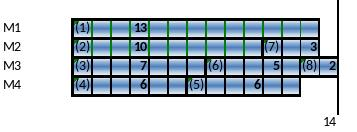
\includegraphics[width=\columnwidth]{Biblio_PCmax_Rendu_exLPT1.jpg}
\caption{Ordonnancement obtenu avec LPT.}
\label{ex:LPTExempleAlgo}
\par}
\end{figure}

\begin{example}
Soit $P=\{13,10,7,6,6,5,3,2\}$, l'ensemble des $p_j$ déjà triés dans
l'ordre décroissant à appliquer sur 4 machines parallèles identiques:

Nous obtenons $C_4^{LPT}(J)=14$ (figure \ref{ex:LPTExempleAlgo}).
\end{example}

% Complexité
% -------------------------------------------------------
\begin{theoreme}
\begin{flushleft}
\begin{tabular}{|p{8cm}p{6cm}|}
% TITRES (pas de titre)
\hline
% Ligne blanche
& \\
% Ligne Complexité en temps
Le tri puis l'affectation coûtent en temps:& $O(n \log n + n \log m)$
\\	% pas de ligne \hline
% RATIO
Le ratio d'approximation:	&	$\Gamma(LPT)\leq \frac{4}{3} - \frac{1}{3m}$
\\
% Ligne blanche
& \\
\hline
\end{tabular}
%pas de legende
\end{flushleft}
\end{theoreme}


% -------------------------------------------------------
% LPT-REV
% -------------------------------------------------------
\subsubsection{LPT-Rev} % (Croce \emph{et al.}, 2018)}

% Présentaion
% ---------------------
Le ratio d'approximation obtenu par LPT (algorithme \ref{algo:LPT})
$(\Gamma(LPT)\leq \frac{4}{3} - \frac{1}{3m})$ est une borne
supérieure que cet algorithme peut atteindre, mais qu'il ne dépassera
jamais.
Chaque utilisation de LPT produira un résultat dont le ratio $\Gamma$
oscillera entre 1 et $\frac{4}{3} - \frac{1}{3m}$.
\bigskip

% figures pour l'explication
% ---------------------
\begin{figure}
{\centering}
% Exemple à gauche
	\begin{subfigure}[b]{0.45\linewidth}
    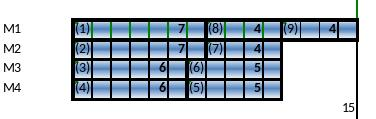
\includegraphics[width=\linewidth]
    {Biblio_PCmax_Rendu_exLPT_Rev1.jpg}
    \caption{Ordonnancement obtenu avec LPT}
  	\end{subfigure}
\hfill% sinon, en fin de page, et pas sur la même ligne
% Exemple optimal à droite
	\begin{subfigure}[b]{0.45\linewidth}
    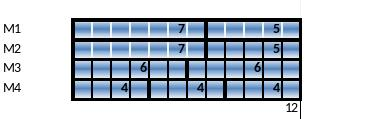
\includegraphics[width=\linewidth]
    {Biblio_PCmax_Rendu_exLPT_Rev2.jpg}
    \caption{Ordonnancement optimal}
  	\end{subfigure}
%CAPTION/FIGURE Complete
  	\caption{LPT, pire cas}
  	\label{fig:LPTExemplePireCas}
\end{figure}

% Exemple pour l'explication
% ---------------------
\begin{example}
\begin{flushleft}
Exemple de pire cas (figure \ref{fig:LPTExemplePireCas}) de LPT (algorithme \ref{algo:LPT})

Soit $P=\{7,7,6,6,5,5,4,4,4\}$, l'ensemble des $p_j$ déjà triés dans
l'ordre décroissant à appliquer sur 4 machines parallèles identiques:
\bigskip
LPT donne le résultat suivant: $C_m^A(J) = 15$
\bigskip

Un ordonnancement optimal aurait été: $C_4^{\star}(J)=12$

Soit une marge de $\frac{15}{12}$

Le ratio d'approximation prévu pour $m=4$:

\[
  \frac{4}{3} - \frac{1}{3m}=\frac{16}{12} - \frac{1}{12}=\frac{15}{12}
\]

Ce cas représente donc un pire cas pour LPT.
\end{flushleft}
\label{ex:LPTExemplePireCas}
\end{example}

\bigskip

% Definitions
% Machine critique
% Job Critique
% ---------------------
\begin{definition}{Job et machine critique}
Le job critique (noté $J^\prime$) est le job qui détermine le
makespan.

La machine critique est la machine qui exécute le job critique.
\end{definition}

% Introduction
% ALGO LPT-Rev Croce et al.
% ---------------------
Croce \emph{et al.}
\cite{della2018longest}, en examinant le comportement de LPT rule,
notamment au niveau du ratio d'approximation, constatent que celui-ci
peut être réduit selon certaines configurations, ou instances du
problème, et rédigent le théorème suivant:

\begin{theoreme}
  LPT a un rapport d'approximation non supérieur à\\
  $\frac{4}{3} - \frac{1}{3(m-1)}$ pour $m \geq 3$ et $n \neq 2m+1$.
\end{theoreme}

\bigskip
LPT atteint la limite de Graham $\frac{4}{3} - \frac{1}{3m}$ pour
$m \geq 2$ et uniquement dans le cas où $n=2m+1$, et la machine
critique traite 3 jobs, tandis que les autres en traitent 2
(ce qui est précisément le cas de l'exemple \ref{ex:LPTExemplePireCas}).


Le rapport $\frac{4}{3} - \frac{1}{3(m-1)}$ est inférieur au
ratio $\frac{4}{3} - \frac{1}{3m}$ (quel que soit le nombre de
machines)

\bigskip

Une modification à l'algorithme LPT rule est apportée afin de placer
le problème \problemGrahamP toujours dans une instance où le ratio
d'approximation est $\leq \frac{4}{3} - \frac{1}{3(m-1)}$.
Cette modification consiste à planifier en premier, le job critique
sur une machine m1.

\bigskip

% Algorithme
% ---------------------
\begin{algorithm}[H]
\DontPrintSemicolon
\KwData{instance de \problemGrahamP, avec $m$ machines, $n$ jobs}
%\Begin{ %inutile ici et rajoute un nuero de ligne

Appliquer LPT ce qui donne un ordonnancement avec
un makespan $z_1$ et $k-1$ jobs sur la machine critique avant le job $J^\prime$
\BlankLine % Petit espace

Appliquer $LPT^\prime = LPT(J^\prime)$
ce qui donne une solution avec un makespan $z_2$
\BlankLine % Petit espace

\Si{  $m=2$ }
{
Appliquer $LPT''=LPT([(J^\prime - k + 1), ...
, J^\prime])$
ce qui donne une solution avec un makespan $z_3$ \\
\Return $\min(z_1,z_2,z_3)$
}
\Sinon
{
\Return $\min(z_1,z_2)$

}
\caption{LPT-Rev\label{algo:LPTRev}}
\end{algorithm}


\bigskip

% Complexité
% -------------------------------------------------------
\begin{theoreme}
\begin{flushleft}
\begin{tabular}{|p{8cm}p{6cm}|}
% TITRES (pas de titre)
\hline
\\
% Ligne blanche
Complexité en temps:	& $O(n \cdot log (n))$
\\
% RATIO
Ratio d'approximation:	&	$\Gamma(LPT-REV)\leq \frac{4}{3} - \frac{1}{3(m-1)}$
\\
% Ligne blanche
& \\
\hline
\end{tabular}
%pas de legende
\end{flushleft}
\end{theoreme}

\subsubsection{Autres algorithmes}

Il existe d'autres propositions basées sur LS, telles que
\begin{itemize}
\item AP de mokotoff\emph{et al.} \cite{mokotoff2004exact}:
AP trie les jobs selon LPT rule (algorithme \ref{algo:LPT}),
partitionne l'ensemble des machines en $r$ sous-ensembles, et définit
une limite que la somme des jobs par machine ne devra pas dépasser.
Les jobs sont attribués selon l'algorithme de LPT rule, sur une
première partition.
Une fois la limite atteinte, les jobs restants sont attribués de la
même façon à une deuxième partition.
Et ainsi de suite.

\item 3-phase de França \emph{et al.} \cite{francca1994composite}:
  Cet algorithme se déroule en 3 phases:
  \begin{enumerate}
  \item Construction: chaque job est affecté aux machines, de telle
    sorte d'obtenir un résultat assez équilibré.
  \item Redistribution: L'équilibre est réajusté, en déplaçant à
    plusieurs reprises un job de la machine la plus chargée, vers la
    machine la moins chargée.
  \item Amélioration: Echange de jobs entre les machines pour
    finaliser l'équilibre des charges de l'ensemble des machines.
  \end{enumerate}
\end{itemize}


\subsection{Bin-Packing} \label{ssec:heuristiquesBinPacking}

Le problème Bin-packing, est semblable au problème \problemGrahamP.
Il consiste à ranger des objets de taille différentes, dans des bacs
identiques, tout en minimisant leur nombre.

L'ensemble des $n$ jobs $J = \{j_1, j_2, \ldots, j_n\}$, et de leurs temps de
traitement $p_j \in P = \{p_1, p_2, ..., p_n\}$, peuvent être vus
respectivement comme:
\begin{itemize}
\item un ensemble d'objets $t_j \in T = \{t_1, t_2, ..., t_n\}$
\item leur taille $L(t_j)$ avec $1 \le j \le n$
\end{itemize}
Une taille maximale $C$ des bacs (ou boites) est donnée.
\bigskip

\begin{definition}{Packing}
  Un packing, est une partition $P<P_1, P_2, ..., P_m>$ tel que
  $L(P_i) \leq C$ avec $1 \leq i\leq m$.
  Le but est de placer les objets $t_j$ dans des bacs $P_i$ de taille
  $C$, de manière à minimiser le nombre de bacs $m$.
\end{definition}

le problème Bin-packing est NP-Complet \cite{Johnson1974WorstCasePB}.

L'idée est d'utiliser le problème Bin-Packing à l'envers, pour
approcher une solution au problème d'ordonnancement.


% -------------------------------------------------------
% MULTIFIT
% -------------------------------------------------------
\subsubsection{Multifit}

% Présentaion
% ---------------------
Coffman \emph{et al.} \cite{coffman1978application} se sont
intéressés à l'algorithme FFD (First Fit Decreasing), un outil de
résolution du problème de Bin-Packing, pour l'adapter au problème
\problemGrahamP.
$FFD(T,C)$ renvoie le nombre de bacs de taille C non vides
nécessaires, et l'arrangement correspondant de l'ensemble $T$ d'objets.

\bigskip
% Principe de l'algorithme
% ---------------------
Soit $T_m^\star = \min\{C:FFD(T,C) \leq m\}$ la plus petite valeur de
$C$ (taille des bacs) qui permet à $T$ d'être pacqué dans $m$ (ou moins)
bacs.

\bigskip


L'idée de MULTIFIT est donc de proposer une valeur pour $C$, faire
tourner $FFD(T,C) $, et réduire à chaque itération cette valeur de $C$
jusqu'à ce que le nombre $m$ de bacs renvoyé par $FFD(T,C) $, alors
devenu insuffisant, augmente à $m+1$ (figure \ref{ex:MULTIFITExempleAlgo}).
Cette valeur charnière de $C$ est $T_m^\star$, qui correspond au
makespan minimum recherché, de l'ordonnancement de l'ensemble $T$ de
jobs sur $m$ machines identiques parallèles.
La difficulté, est de proposer une première valeur de $C$ pas trop
éloignée de la valeur recherchée, afin de réduire au maximum le nombre
d'itérations.

La méthode utilisée est une recherche dichotomique.
Après avoir défini les bornes supérieure
$C_u = \max\{\frac{2}{m} \cdot L(T), \max_i\{L(T_i)\} \}$ et
inférieure $C_l = \max\{\frac{2}{m} \cdot L(T), \max_i\{L(T_i)\} \}$
de départ, FFD est exécuté avec le milieu $C_d = \frac{C_u + C_l}{2}$.
si $FFD(T,C_d)\le m$ alors la nouvelle fourchette de recherche devient
$C_u = C_d$ et $C_l$, sinon (si $FFD(T,C_d)> m$) alors la nouvelle
fourchette devient $C_u$ et $C_l = C_d$.
Un nombre d'itérations $k$ et donné à l'exécution de MULTIFIT, estimé
en fonction de la taille du problème ($n$ et $m$).
Mais même pour un problèmes de grande taille, le résultat ne change
plus après $7$ itérations.
Il est donc inutile d'utiliser $k>7$.

\begin{figure}
\centering{
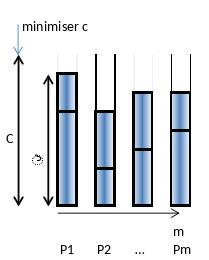
\includegraphics[width=6.5cm]{Biblio_PCmax_Rendu_exMULTIFIT1.jpg}
\caption{Fonctionnement de FFD et principe de MULTIFIT.}
\label{ex:MULTIFITExempleAlgo}
\par}
\end{figure}

\bigskip

% Algorithme
% ---------------------
\begin{algorithm}[H]
\DontPrintSemicolon
\KwData{T un ensemble de jobs

m, un nombre de processeurs

borne supérieure: $Cu[T,m] = \max\left\{\frac{2}{m} \cdot L(T), \max_i\{L(T_i)\} \right\}$

borne inférieure: $Cl[T,m] = \max\left\{\frac{1}{m} \cdot L(T), \max_i\{L(T_i)\} \right\}$

k un nombre d'itérations
}

\BlankLine % Petit espace
La recherche de $T_m^\star$ s'effectue par dichotomie sur $k$ itérations

\BlankLine % Petit espace
Après les $k$ itérations, MULTIFIT \Return {$Cu(k)$} \\
\tcp{qui correspond à la plus petite valeur de $C$
pour laquelle $FFD[T,C] \leq m$}

\caption{MULTIFIT\label{algo:MULTIFIT}}
\end{algorithm}

\bigskip

% Complexité
% -------------------------------------------------------
\begin{theoreme}
\begin{flushleft}
\begin{tabular}{|p{8cm}p{6cm}|}
% TITRES (pas de titre)
\hline
% Ligne blanche
& \\
% Ligne Complexité
Tri puis $k$ FFD coûtent en temps: & $O(n \log n + kn \log m)$
\\	% pas de ligne \hline
% Ligne blanche
& \\
% RATIO
Ratio \cite{lee1988multiprocessor}:& $\Gamma(MULTIFIT) \leq 1,220 + 2^{-k}$
\\
% Ligne blanche
& \\
\hline
\end{tabular}
%pas de legende
\end{flushleft}
avec $k$ le nombre d'itérations pour la recherche dichotomique.
\end{theoreme}

Généralement, MULTIFIT donne des résultats très satisfaisant avec $k = 7$


% -------------------------------------------------------
% COMBINE
% -------------------------------------------------------
\subsubsection{Combine}

% Présentaion
% ---------------------
Lee \emph{et al.}, \cite{lee1988multiprocessor} ont l'idée
d'utiliser LPT (algorithme \ref{algo:LPT}) pour réduire les bornes de départ
et ainsi optimiser MULTIFIT (algorithme \ref{algo:MULTIFIT}) dans un
algorithme nommé COMBINE.

\bigskip
soient
\begin{align*}
&\textnormal{la moyenne des poids des jobs par processeur} &A &= \sum_{i=1}^{n}(\frac{P_i}{m})\\
&et &M &= C_m^{lpt}(J) \\
& &M^\star &= C_m^\star(J)
\end{align*}

COMBINE, améliore certains points de l'algorithme MULTIFIT en se basant
sur les principes suivants:
\begin{itemize}
\item Le résultat $M$ obtenu par LPT, est forcément supérieur ou égal
  à $M^\star$, soit $M \ge M^\star$.
  COMBINE utilise donc $M = C_m^{lpt}(J)$ comme borne supérieure $C_u$
  de départ pour la recherche dichotomique utilisée par MULTIFIT.
  celle-ci est beaucoup plus proche du résultat optimal que la borne
  supérieure de départ $2\cdot A$ utilisée à l'origine par MULTIFIT.
\item Si le résultat $M$ obtenu par LPT est tel que
  $M \geq 1,5\cdot A$ alors $M=M^\star$.
  Il n'est donc pas nécessaire de poursuivre la recherche.
\item Au lieu de prédéterminer un nombre d'itérations, COMBINE utilise
  une condition d'arrêt de la recherche dichotomique, en fonction de
  l'écart entre les deux bornes.
  COMBINE stoppe la recherche dès que $C_u - C_l \le \alpha \cdot A$.
  Les tests de COMBINE ont été effectués avec $\alpha = 0,005$
\end{itemize}


\bigskip
% Algorithme
% ---------------------
\begin{algorithm}[H]
\DontPrintSemicolon
\KwData{instance de \problemGrahamP, avec $m$ machines, $n$ jobs, et un coefficient $\alpha (0,005)$ }

A = $\sum_{i=1}^{n}(\frac{P_i}{m})$ \;
M $\leftarrow C_m^{lpt}(J)$ \;
\Si {$M \geq 1,5 \cdot A$}
 {
 	$M^\star = M$ \;
 }
\Sinon
 {
	$C_u \leftarrow M$					\;
	$C_l \leftarrow \max \left\{\frac{M}{\frac{4}{3}-\frac{1}{3 \cdot m}},P_1,1 \right\}$ \;
	\Tq {$C_u - C_l > \alpha \cdot A$}
	 {
	 appliquer MULTIFIT \;
	 } \tcp{on arrête lorsque $C_u - C_l \leq \alpha \cdot A$}
 }

\caption{COMBINE}
\label{algo:COMBINE}
\end{algorithm}


\bigskip

% Complexité
% -------------------------------------------------------
\begin{theoreme}
\begin{flushleft}
\begin{tabular}{|p{8cm}p{6cm}|}
% TITRES (pas de titre)
\hline
% Ligne blanche
& \\
% Ligne Complexité
Complexité en temps: & $O(n \log n + kn \log m)$
\\	% pas de ligne \hline
% Ligne blanche
& \\
% RATIO
Ratio \cite{gupta2001listfit}: & $\Gamma(COMBINE) \leq \frac{13}{12} + 2^{-k}$
\\
% Ligne blanche
& \\
\hline
\end{tabular}
%pas de legende
\end{flushleft}
avec $k$ le nombre d'itérations pour la recherche dichotomique.
\end{theoreme}

Concernant la complexité, pour atteindre
$C_u - C_l \leq \alpha \cdot A$, généralement, 6 itérations suffisent
($k=6$).
Mais COMBINE a déjà exécuté une fois LPT (donc $k=7$).


% -------------------------------------------------------
% LISTFIT
% -------------------------------------------------------
\subsubsection{Listfit}

% Présentaion
% ---------------------
Gupta \emph{et al.}, \cite{gupta2001listfit}, ont aussi l'idée
d'utiliser MULTIFIT (algorithme \ref{algo:MULTIFIT}), afin de réaliser l'algorithme
LISTFIT.

Celui-ci sépare la liste des travaux en 2 sous-listes, traitées soit
dans un ordre LPT (Longest Time Processing), soit dans un ordre SPT
(Shortest Time Processing).
Puis LISTFIT combine ces 2 sous-listes en appliquant MULTIFIT à chaque
itération.
% \lp{Expliquer l'intérêt, donner une idée intuitive}

\bigskip

% Algorithme
% ---------------------
\begin{algorithm}[H]
\DontPrintSemicolon
\KwData{n, m, $p_j$ for $j=1, \ldots, n$}

%STEP 1
Soient $r=0$, $q=0$, $C_{\max}=C_{\max}(LPT)$: le makespan obtenu par LPT

\BlankLine % Petit espace
\Tq {$q<2$}
{
	$r = 0$ \;
	$q = q + 1$ \;
	\Tq {r < 2}
	{
		$ r = r + 1$ \;
		Soient $\Phi_q = \varnothing$, A = $\{1,...,n\}$, $B = \varnothing$ \;
		Soit  $\omega_r$ la séquence des jobs de la liste des jobs $A$
		triés selon l'ordre $r$. \;
		\tcp{Si $r = 1$ alors tri en SPT,}
		\tcp{Si $r = 2$ alors tri en LPT.}
		\Tq{$A \neq \varnothing$}
		{
			$\alpha=C_{\max}(MULTIFIT)$: le makespan obtenu via MULTIFIT,
			avec $\sigma = \Phi_q \cdot \omega_r$
                        ($1^{ère}$ étape de MULTIFIT) \;
			\Si {$C_{\max}>\alpha$}
				{
				$C_{\max} = \alpha$ \;
				\Pour {$h=1$ à $m$}
					{$\gamma_h = \pi_h$}
				}
			\Si {$A \neq \varnothing$}
			{
				Retirer le dernier job de $\omega_r$ et le placer dans $B$ \;
				Mettre à jour $A$, $\Phi_q$, $\omega_r$. \;
				$\sigma = \Phi_q \cdot \omega_r$.
			}
		}
	}
}
\tcp{L'ordonnancement où les jobs en $\gamma_h$ sont traités par la machine $h$}
\tcp{est une solution approximative du problème \problemGrahamP }
\tcp{avec un makespan $C_{\max}$.}

\caption{LISTFIT}
\label{algo:LISTFIT}
\end{algorithm}

\bigskip
% Complexité
% -------------------------------------------------------
\begin{theoreme}
\begin{flushleft}
\begin{tabular}{|p{8cm}p{6cm}|}
% TITRES (pas de titre)
\hline
% Ligne blanche
& \\
% Ligne Complexité
Complexité en temps:& $O(n^2 \log(n) + k \cdot n^2 \log(m))$
\\	% pas de ligne \hline
% Ligne blanche
& \\
% RATIO
Ratio \cite{gupta2001listfit} & $\Gamma(LISTFIT) \leq \frac{13}{12} + 2^{-k}$
\\
% Ligne blanche
& \\
\hline
\end{tabular}
%pas de legende
\end{flushleft}
avec $k$ le nombre d'itérations pour la recherche dichotomique.
\end{theoreme}


\subsection{Approche gloutonne} \label{ssec:heuristiquesGloutonne}

% -------------------------------------------------------
% SLACK
% -------------------------------------------------------
\subsubsection{Slack} %(Croce \emph{et al.}, 2018)}

% Présentaion
% ---------------------
Croce \emph{et al.} \cite{della2018longest}, en effectuant la preuve
d'une borne d'approximation pour le
développement de LPT-Rev (algorithme \ref{algo:LPTRev}), ont mis en évidence l'importance des différences de temps entre les jobs, 
ainsi que le regroupement de ceux-ci en sous-ensembles.

En effet, lorsque le nombre de jobs $n =2 \cdot m + 1$, que la différence entre $p_1 - p_m < p_{2 \cdot m + 1}$ et que 
$p_{2 \cdot m + 1}$ est planifié en premier (sur $m_1$) 
alors la machine critique exécute $p_{m+1}$, $p_m$ et $p_{2 \cdot m}$
(donc $C_m^{LPT \prime}(J) = p_{m+1}$+$p_m$+$p_{2 \cdot m} $), 
et le ratio d'approximation tombe à 
$\frac{6}{7}$ au lieu de 
$\frac{4}{3} - \frac{1}{2 \cdot m -1)}$, 
soit $1.1666 \ldots$ \\
$\frac{6}{7} < \frac{4}{3} - \frac{1}{2 \cdot m -1)}$ avec $m \geq 4$.

Il faut donc se placer dans cette instance en adoptant la stratégie gloutonne suivante :


\bigskip

% Algorithme Slack
% ---------------------
\begin{algorithm}[H]
\DontPrintSemicolon
% \KwData{une instance ...}

%Etape 1
trier la liste des jobs dans l'ordre décroissant des temps nécessaires de traitements \;
%ETAPE 2
réindexer les jobs, de manière à obtenir $p_1 \geq p_2 \geq ... \geq p_n$ \;
%ETAPE 3
découper l'ensemble obtenu en $\lceil \frac{n}{m} \rceil$ tuples de $m$ jobs (ajout
de jobs ``dummy'' de taille nulle pour le dernier tuple, si $n$ n'est
pas un multiple de $m$) \;
%ETAPE 4
considérer chaque tuple avec la différence de temps (SLACK) entre le
premier job du tuple et le dernier.
\begin{align*}
\{ &\{1, ..., m\} &\{m+1,..., 2 \cdot m\} &... \} \\
   &p_1 - p_m     &p_{m+1}-p_{2 \cdot m}  &...
\end{align*} \;
%STEP 5
trier les tuples par ordre décroissant de ``Slack'' et ainsi former un nouvel ensemble
\tcp{e.g: $\{ \{m+1,..., 2 \cdot m\} \{1, ..., m\}\}$ si $p_{m+1} - p_{2 \cdot m} > p_1 - p_m$.}
%STEP 6
appliquer l'ordonnancement (affectation à la machine la moins chargée à
ce moment là) à l'ensemble ainsi obtenu.
\caption{SLACK\label{algo:SLACK}}
\end{algorithm}

\bigskip
% Complexité
% -------------------------------------------------------
\begin{theoreme}
\begin{flushleft}
\begin{tabular}{|p{8cm}p{6cm}|}
% TITRES (pas de titre)
\hline
% Ligne blanche
& \\
% Ligne Complexité
Complexité en temps:& $O(n \cdot log (n))$
%	\\	% pas de ligne \hline
%	% Ligne blanche
%	& \\
%	% RATIO
%	Ratio \cite{gupta2001listfit} & $\Gamma(LISTFIT) \leq \frac{13}{12} + 2^{-k}$
\\
% Ligne blanche
& \\
\hline
\end{tabular}
%pas de legende
\end{flushleft}
\end{theoreme}


\section{Programmation linéaire} \label{sec:programmationLineaire}

L'ordonnancement, et plus particulièrement \problemGrahamP, s'inscrit
parfaitement dans l'énoncé d'un problème de programmation linéaire.
En effet, la fonction objectif, i.e.\ minimiser le makespan, ainsi que
les contraintes sont des fonctions linéaires.
Toutefois, les variables, et le résultat attendu, sont discrets, ce qui
rend la résolution du problème nettement plus difficile comparé à une
programmation linéaire à variables continues.
Ces algorithmes, donnent une solution faisable exacte.

\subsection{PA} %(Mokotoff)}

Mokotoff \cite{mokoto1999scheduling} présente un algorithme basé sur
la formulation de la programmation linéaire en utilisant des
variables booléennes d'affectation des jobs à une machine, i.e.\
$x_{ij}$ est égal à 1 si le job $j_j$ est affecté à la machine $m_i$, ou
0 dans le cas contraire.

% Présentation
% ---------------------
\bigskip
La minimisation du makespan peut être posée ainsi:

Minimiser $y$ tel que:

\begin{itemize}
\item $\sum_{i=1}^{m}x_{ij}=1$ \quad pour $1 \leq j \leq n$

Sur toutes les machines, au moins un et un seul $x_j$ est égal à 1.
Un job est affecté à une et une seule machine.

\item $y-\sum_{j=1}^{n}p_j \cdot x_{ij} \geq 0$ \quad pour $1 \leq i \leq m$

Pour une machine donnée, la somme des temps est inférieure ou égale à $y$.
\end{itemize}

\bigskip
Où la valeur optimale de $y$ est $C_{\max}$
et
\[
  x_{ij} =
  \begin{cases}
    1 \textnormal{ si le job $j_j$ est affecté à la machine $m_i$}\\
    0 \textnormal{ sinon.}\\
  \end{cases}
\]

Le programme linéaire est donc composé de
\begin{itemize}
\item $n \cdot m + 1$ variables (les variables $x_{ij}$ et la variable $y$)
\item $n+m$ contraintes
\end{itemize}

La zone $F$ peut être définie ainsi:
\[
  F=\{ (x,y) : x \in B^{n \cdot m}, y \in \mathbb{R_+} : \sum_{i=1}^{m} x_{ij}=1 \forall j;
y-\sum_{j=1}^{n} p_j \cdot x_{ij} \geq 0 \forall i \}
\]

avec
\[
B=\begin{bmatrix}
x_{11}& &x_{n1}\\
& \ddots & \\
x_{1m}& &x_{nm1}
\end{bmatrix}.
\]

Le polytope $P$ relatif à $F$ est défini ainsi:
\[
  P=\{ (x,y) : x \in \mathbb{R_+}^{n \cdot m}, y \in \mathbb{R_+} : \sum_{i=1}^{m} x_{ij}=1 \forall j;
  y-\sum_{j=1}^{n} p_j \cdot x_{ij} \geq 0 \forall i	\}
\]

Il est possible de construire un ensemble fini d'\textbf{inégalités}
\[
  Ax+Dy \leq \overline{b}
\]
telles que
\[
  \min \{y : (x,y) \in F \} = \min \{y : x \in \mathbb{R_+}^{n \cdot m}, y \in \mathbb{R_+} Ax+Dy \leq \underline{b}
\]
% \ensuremath{^\circ} pour le symbole °
NB: une solution
$(x \ensuremath{^\circ} , y\ensuremath{^\circ}) \in P$ doit être
exclue (car n'est pas un vecteur entier) si
$(x\ensuremath{^\circ}, y\ensuremath{^\circ}) \notin P $.

\bigskip

Des \textbf{inégalités transitoires} peuvent être générées (nombre
maximum de jobs par machine)
\[
  \sum_{j \in S_i} x_{ij} \leq L_i \quad (L_i = h-1 \iff S_{j_h} > LB
  \textnormal{ et } S_{j_{(h-1)}} \leq LB)
\]
LB: borne inférieure.

\bigskip

Pour un problème \problemGrahamP, même de taille modeste, le nombre de
variables et contraintes est très important, et certaines sont
inutiles.
L'algorithme va donc utiliser la méthode des plans sécants (Cutting
Plane Method).
\`A chaque itération , des inégalités valides sont générées, puis une
relaxation est exécutée, jusqu'à l'obtention d'une solution faisable.

\bigskip
% Algorithme PA
% ---------------------
\begin{algorithm}[H]
\DontPrintSemicolon

Déterminer la borne inférieure $(LB)$ suivant l'algorithme de
McNaughton \cite{mcnaughton1959scheduling}.\;

Déterminer la borne supérieure $UB$ suivant l'heuristique LPT
(algorithme \ref{algo:LPT}).\;

\Si{$LB=UB$}{
  \Return la solution optimale est trouvée par l'heuristique LPT
}

\Repeter{Génération des d'inégalités impossible}
{
	Résoudre le programme de relaxation linéaire avec $C_{max} = LB$
	
	\Si {la relaxation est possible}
	{
	
		\Si {la solution obtenue est entière (donc faisable)}
		{
		\Return la solution obtenue qui est optimale
		}
		\Sinon
		{
		Générer des nouvelles inégalités 
		(inégalités et/ou inégalités transitoires) et les ajouter à la 
		nouvelle relaxation linéaire
		}
	}
	\Sinon
	{
	incrémenter $LB$ d'une unité
	}	


}
\Return Résoudre le problème avec un algorithme Branch\&Bound
.\;
\caption{PA\label{algo:PA}}
\end{algorithm}


\section{Approximation} \label{sec:approximation}

Une catégorie d'algorithmes fournit une garantie d'approche.
Notamment les PTAS (Schéma d'Approximation en Temps Polynomial).

Un PTAS est un algorithme qui calcule, pour tout $\epsilon > 0$ donné,
une solution proche à un facteur $(1+\epsilon)$ pour un problème de
minimisation, ou $(1-\epsilon)$ pour un problème de maximisation, de
l'optimal, en temps polynomial dépendant de $\epsilon$.


\subsection{PTAS dual} \label{ssec:approximationPTAS} % (Hochbaum \emph{et al.})}

Hochbaum \emph{et al.}\ \cite{hochbaum1987using} proposent le
premier PTAS adapté au problème \problemGrahamP.
Cette approche s'appuie aussi sur le problème semblable à
\problemGrahamP, celui du bin-packing et prend MULTIFIT
(algorithme \ref{algo:MULTIFIT}) comme réflexion de départ.
Le problème bin-packing est posé différemment:

Soient:
\begin{itemize}
\item un ensemble d'objets $t_j \in T = \{t_1, t_2, ..., t_n\}$;
\item leur taille $L(t_j)$ avec $1 \le j \le n$ et $0 \le L(t_j) \le 1$.
\end{itemize}
Une taille maximale $C$ des bacs (ou boites).

$T^{\star}(T)$, définit plus haut, correspond au bin-packing idéal, et donc,
au nombre minimum de bacs nécessaires pour l'organisation des pièces
de l'ensemble $T$.
Le but de l'algorithme proposé est de construire un arrangement
bin-packing,
qui utilise au plus $T^{\star}_m$ bacs, remplit
avec des pièces totalisant une taille au plus de $1+ \epsilon$,
et ainsi donner une réponse au problème \problemGrahamP en temps polynomial.

Le problème bin-packing et \problemGrahamP sont reliés de la façon suivante:
$T^{\star}(\frac{J}{C}) \le m$ si et seulement si $C^{\star}_m(J) \le C$.
Donc la taille minimale des bacs, $C^{\star}$, correspondant au délai
idéal makespan est telle que $T^{\star}(\frac{J}{C^{\star}}) \le m$.

Nous sommes en présence de deux paramètres critiques:
\begin{itemize}
\item $m$ le nombre de machines parallèles identiques;
\item $C$ la taille des bacs, et aussi, le makespan recherché.
\end{itemize}
Il y a donc deux problèmes d'optimisation,
dont l'un consiste à fixer le premier paramètre pour optimiser l'autre,
et inversement, fixer l'autre pour optimiser le premier.
Ce qui constitue un problème de reconnaissance (ou décision) à deux
paramètres $R(p_1, p_2)$.

\paragraph{Problème primal et approximation $\epsilon-$primal}

Soit le problème primal $(J,\bar{p_1})$
où $p_1$ est donné en paramètre et $p_2$ est optimisé.

La valeur optimale est $OPT_P(J,\bar{p_1})$.

Soit l'algorithme d'approximation $\epsilon-$primal pour le problème
primal, qui donne comme résultats:

\begin{itemize}
\item pour le premier paramètre $p_1$ une valeur inférieure ou égale à $\bar{p_1}$;
\item pour le deuxième paramètre $p_2$ une valeur $PRIMAL_{P,\epsilon} \le (1+\epsilon)\cdot OPT_P(J,\bar{p_1})$.
\end{itemize}

\paragraph{Problème dual et approximation $\epsilon-$dual}

Soit le problème primal $(J,\bar{p_2})$
où $p_2$ est donné en paramètre et $p_1$ est optimisé.

La valeur optimale est $OPT_D(J,\bar{p_2})$.

Soit l'algorithme d'approximation $\epsilon-$dual pour le problème
dual, qui donne comme résultats:

\begin{itemize}
\item pour le premier paramètre $p_1$ une valeur $DUAL_{D,\epsilon}(J, \bar{p_2})\le OPT_D(J,\bar{p_2})$;
\item pour le deuxième paramètre $p_2$ une valeur $ \le (1+\epsilon)\cdot \bar{p_2}$.
\end{itemize}

\bigskip

Trouver un algorithme $\epsilon-$primal pour le problème primal
peut être réduit à trouver un algorithme $\epsilon-$dual pour le problème dual.

Trouver un algorithme d'approximation $\epsilon-$dual peut être
réduit à trouver un algorithme
d'approximation $\epsilon-$dual pour une instance du problème où la
taille des pièces sont strictement supérieures à $\epsilon$.

 %\lp{C'est dommage que par la suite te te sois concentrer sur
 %  l'expression à partir des bins sans conserver le lien avec le
 %  problème $P||C_{\max}$, en particulier pour les algos}

L'intervalle de la taille des pièces (devenu $]\epsilon, 1]$) est
découpé en S = $\lceil \frac{1}{\epsilon^2}\rceil$ sous intervalles
de tailles identiques
$]\epsilon = l_1, l_2], ]l_2, l_3], \ldots , ]l_S, L_{S+1}=1]$.
Chaque bac $P_i$, sera rempli au maximum avec
$\lfloor \frac{1}{\epsilon} \rfloor$ pièces.

Soit $x_k$ avec $1 \le k \le S$ le nombre de pièces d'un bac dont la
taille est comprises dans $]l_k, l_{k+1}]$.
Chaque $x_k$ peut prendre une valeur dans l'intervalle
$[0,\frac{1}{\epsilon}[$

La configuration d'un bac $P_i$ peut être donnée par un s-tuple $(x_1, x_2, \ldots, x_S)$.
Soit $cf(x_1, \ldots ,x_S)$ une configuration dite faisable si 
$\sum_{k=1}^{S}x_k \cdot l_k \le 1$ 
avec $l_k$ de $]l_k, l_{k+1}]$.


Nous avons donc

\begin{align*}
L(P_i) & \le \sum_{k=1}^{S}x_k \cdot l_{k+1} \\
& \le \sum_{k=1}^{S}x_k \cdot (l_k+\epsilon^2) \\
& = \sum_{k=1}^{S}x_k \cdot l_k  +  \epsilon^2 \cdot \sum_{k=1}^{S}x_k \\
& \le 1 + \epsilon^2 \cdot \frac{1}{\epsilon} \\
& = 1 + \epsilon
\end{align*}

Soit $b_k$ avec $1 \le k \le S$ le nombre de pièces utilisées dans
tous les bacs dont la taille appartient à $]l_k, l_{k+1}]$.

Soit $Bins(b_1, b_2, \ldots, b_S)$ le nombre minimum de bacs
nécessaires, lorsqu'il y a $b_k$ pièces de taille $l_k$, et
considérons que le premier bac soit rempli. Nous obtenons:

\[
  Bins(b_1, b_2, \ldots, b_S) = 1 + \underset{cf(x_1, \ldots ,x_S)}{\min} Bins(b_1-x_1, b_2-x_2, \ldots, b_S-x_S)
\]


Ce qui est résolu par programmation dynamique.
Il existe 2 versions optimisées d'algorithmes pour
$\epsilon = \frac{1}{5}$ et
$\epsilon = \frac{1}{6}$.

\bigskip

$k-bin$ désigne un bac rempli avec $k$ pièces.

$L[u_1, \ldots, u_k]$ désigne l'ensemble des
$k$ pièces distinctes $\{i_1, \ldots, i_k\}$
où $i_l$ est la plus grande pièce, de taille au plus $u_l$,
et où $u_1 \leq u_2 \leq \ldots \leq u_k$ et
$p_{i_1} \leq p_{i_2} \leq \ldots \leq p_{i_k}$.


% Algorithme 1/5
% ---------------------
\begin{algorithm}[H]
\DontPrintSemicolon

Tant qu'il y a $1$ pièce $j$ avec $p_j \in [0,6, 1]$, emballer j avec
$L[1 - p_j]$, si cette pièce existe.
Emballer $j$ toute seule sinon.

\BlankLine % Petit espace
Tant qu'il y a $2$ pièces $i$, $j$ avec $p_i, p_j \in [0,5, 0.6[$,
emballer $i$ et $j$ ensembles.

\BlankLine % Petit espace
\tcp{Chaque pièce restante a une taille inférieure à 0.5}
Tant qu'il existe $3$ pièces, dont la plus grande fait au moins 0.4,
trouver $L[0.3,0.4,0.5]$ et les pacquer ensembles.

\BlankLine % Petit espace
Tant qu'il existe des pièces dont la taille est dans [0.4,0.5[, pacquer
les $2$ plus grandes ensembles.

\BlankLine % Petit espace
\tcp{Chaque pièce restante a une taille inférieure à 0.4}
Prendre la plus petite pièce des pièces restantes. Si $p_j > 0.25$,
alors pacquer le reste des pièces en 3-bin.
Sinon, $p_j = 0.25 - \delta$ pour $\delta \geq 0$.
Si $3$ autres pièces existent, pacquer $j$
 avec $L[0.25, \frac{+\delta}{3}, 0.25 + \delta, 0.25 + 3 \cdot \delta]$.
Sinon, pacquer le reste dans 3-bin.


\caption{PTAS $\frac{1}{5}$-dual}
\label{algo:PTASDual1_5}
\end{algorithm}

\bigskip

% Algorithme 1/6
% ---------------------
\begin{algorithm}[H]
\DontPrintSemicolon

Tant qu'il existe une pièce $j$, telle que $p_j \in (\frac{2}{3},1)$,
emballer $p_j$ avec $L[1-p_j]$.

\BlankLine % Petit espace
Estimer le nombre total de 1-bin ou 2-bin d'une solution optimale du
reste de l'instance.
Pour chacun de ces bacs, l'emballer avec $L[\frac{1}{2}, \frac{2}{3}]$
si de telles pièces existent, sinon, l'emballer avec $L[\frac{2}{3}]$.

\BlankLine % Petit espace
\tcp{Pour le reste de la procédure, seuls les bacs qui ont }
\tcp{au moins $3$ pièces sont considérés.}

\BlankLine % Petit espace
\tcp{Chaque pièce restante a une taille inférieure à $\frac{2}{3}$}
Pour chaque pièce $j$ restante, avec une taille $\frac{1}{2}+\delta;
\delta \geq 0$, emballer $j$ avec $L[\frac{1}{4}-\frac{\delta}{2},
\frac{1}{3}-\delta]$.

\BlankLine % Petit espace
\tcp{Chaque pièce restante a une taille inférieure à $\frac{1}{2}$}
Estimer le nombre de 4-bin qui contient une pièce dont la taille est
dans l'intervalle $[\frac{5}{12}, \frac{1}{2}[$ dans un packing
optimal. Pacquer chaque bac avec $L[ \frac{7}{36}, \frac{5}{24},
\frac{1}{4}, \frac{1}{2}]$.

Pour chaque pièce restante de taille
$\frac{5}{12}+\delta, \delta \geq 0$, l'emballer dans un 3-bin avec
$L[\frac{7}{24}-\frac{\delta}{2}, \frac{5}{12}-\delta]$.

\BlankLine % Petit espace
\tcp{Chaque pièce restante a une taille inférieure à $\frac{5}{12}$}
Estimer le nombre de 3-bin d'une solution optimale pour le reste de
l'instance. Pour chacun d'eux, le pacquer avec $L[\frac{1}{3},
\frac{5}{12}, \frac{5}{12}]$.

\BlankLine % Petit espace
\tcp{Pour le reste de la procédure, seuls les bacs qui ont }
\tcp{au moins $4$ pièces sont considérés.}

Pour chaque pièce $j$ de taille $\frac{1}{3}+\delta, \delta \geq 0$,
emballer $i$
avec $L[\frac{2}{9}-\frac{\delta}{3},
        \frac{1}{4}-\frac{\delta}{2},
        \frac{1}{3}-\delta]$.

\BlankLine % Petit espace
\tcp{Chaque pièce restante a une taille inférieure à $\frac{1}{3}$}
Estimer le nombre de 5-bin qui contienne une pièce
dont la taille est comprise dans l'intervalle
$[\frac{7}{24},\frac{1}{3}[$ d'une solution optimale.
Emballer de tels bacs avec
$L[\frac{17}{96},
   \frac{13}{72},
   \frac{9}{48},
   \frac{5}{24},
   \frac{1}{3}]$.

Tant qu'il existe des pièces dont la taille est supérieure à $\frac{7}{24}$
Prendre la plus grande pièce de taille $p_j = \frac{7}{24}+\delta, \delta \geq 0$.
Pacquer i avec
$L[\frac{17}{72}-\frac{\delta}{3},
   \frac{13}{48}-\frac{\delta}{2},
   \frac{7}{24}+\delta]$.

Considérer la plus petite pièce $j$.
Si $p_j>\frac{1}{5}$, emballer les pièces restantes à raison de $4$ pièces par bac.
Si $p_j=\frac{1}{5}-\delta, \delta \geq 0$, pacquer $j$ avec
$L[\frac{1}{5}+\frac{\delta}{4},
   \frac{1}{5}+\frac{2 \cdot \delta}{3},
   \frac{1}{5}+\frac{3 \cdot \delta}{2},
   \frac{7}{24}]$.

\BlankLine % Petit espace



\caption{PTAS $\frac{1}{6}$-dual}
\label{algo:PTASDual1_6}
\end{algorithm}

\bigskip

% Complexité
% -------------------------------------------------------
\begin{theoreme}
\begin{flushleft}
\begin{tabular}{|p{8cm}p{6cm}|}
% TITRES (pas de titre)
\hline
% Ligne blanche
& \\
% Ligne Complexité
Complexité en temps:& \\
général&
	$ O(( \frac{n}{\epsilon})^\frac{1}{\epsilon ^ 2})$\\
pour $ \epsilon = \frac{1}{5}$ &
	$O(n \cdot (k + \log(n)))$ \\
pour $ \epsilon = \frac{1}{6}$ &
	$O(n \cdot (k \cdot m^4 + \log(n)))$

\\	% pas de ligne \hline
% Ligne blanche
& \\
% RATIO
Ratio & \\
général &
	$\Gamma(dual PTAS) = 1 + \epsilon$\\

pour $ \epsilon = \frac{1}{5}$ &
	$\Gamma(\frac{1}{5}$dual PTAS$) = \frac{1}{5} + 2^{-k}$\\

pour $ \epsilon = \frac{1}{5}$ &
	$\Gamma(\frac{1}{6}$dual PTAS$) = \frac{1}{6} + 2^{-k}$
\\
% Ligne blanche
& \\
\hline
\end{tabular}
%pas de legende
\end{flushleft}
avec $k$ le nombre d'itérations qui a été nécessaire pour terminer l'algorithme.
\end{theoreme}


\subsection{Autres algorithmes}

Il existe d'autres PTAS, ou utilisant des PTAS, tels que:
\begin{itemize}
\item HI-Pcmax de Alvim \emph{et al.} \cite{alvim2004hybrid}.
  Cet algorithme se déroule en 3 phases:
  \begin{enumerate}
  \item Utilisation d'un PTAS MTSS pour affecter les jobs aux machines
    et proposer une première solution $S$.
  \item Utilisation du PTAS de Hauchbaum \emph{et al.}
    (algorithmes \ref{algo:PTASDual1_5}, \ref{algo:PTASDual1_6}) pour
    proposer une deuxième solution $S^\prime$
    et comparaison des deux solutions $S$ et $S^\prime$.
  \item Utilisation de LPT rule (algorithme \ref{algo:LPT}) et
    comparaison de cette solution avec la meilleure des solutions
    précédente.
  \end{enumerate}

\item PTAS GPU-DP de Ghalami \emph{et al.} \cite{li2018gpu}:
  un PTAS optimisé pour l'exécution en GPU.

\item PTAS DP de Ghalami \emph{et al.}
  \cite{ghalami2019scheduling}: cet algorithme est basé sur la
  formulation de PTAS dual de Hochbaum \emph{et al.}
  et utilise le solveur CPLEX pour résoudre cette formulation.
\end{itemize}


\section{Autres approches} \label{sec:autresApproches}

D'autres pistes sont explorées dans la littérature, notamment à l'aide
de réseaux de neurones, d'algorithmes branch\&bound, ou via
l'utilisation de méta-heuristiques\footnote{Les heuristiques sont
spécifiques à un problème. il est nécessaire d'en déterminer une
nouvelle à chaque nouveau problème. Les méta-heuristiques rassemblent
des concepts permettant de définir des heuristiques et ainsi s'adapter
à de nombreux problèmes.}, telles que les algorithmes génétiques.
Ces techniques complexes, et pour l'instant très coûteuses en temps,
sortent en partie du cadre de cette bibliographie (pour exemple Min
\emph{et al.}~\cite{min1999genetic}).

En revanche, et à l'instar du problème bin-packing, le problème de
partitionnement de nombres est similaire à \problemGrahamP,
et fait l'objet d'investigations.

\subsection{Partitionnement de nombres}
\label{ssec:autresApprochesPartitionnement}

Le problème \problemGrahamP peut être vu comme le problème de
partition ou partitionnement de nombres (Npp, \emph{Number Paritioning
Problem}).
En effet, ce problème consiste à partitionner un ensemble de $n$ nombres
dans $m$ sous-ensembles, tout en minimisant la somme des nombres de
chaque sous-ensembles.
Ce problème est NP-difficile.

\subsubsection{LDM}
% \todo{FCO: Rappels, Lipshitz, fonction densité, triangulaire pas pertinent pour l'instant}


Karmarkar \emph{et al.}
\cite{karmarkar1982differencing} posent le problème de partition
d'ensembles suivant: soit un ensemble fini
$P=\{p_1, p_2, \ldots, p_n\}$ de $n$ nombres réels à partitionner dans $m$
sous-ensembles $m_1, m_2, \ldots, m_m$ de manière à minimiser
$D(m_1, m_2, \ldots, m_m) = \max_i \left\{ \sum_{p_j \in m_i}p_j
\right\} - \min_i \left\{ \sum_{p_j \in m_i}p_j \right\}$

Le principe de l'algorithme consiste à remplacer les deux plus grands
nombres de l'ensemble de $n$ éléments de départ (les plus importants, ou
\textbf{Largest}) par leur différence (opération appelée
Differentiation, ou \textbf{Differencing}), donnant ainsi un nouvel
ensemble de $n-1$ éléments.
D'où le nom LDM, ou Largest Differencing Method.


La réflexion est tout d'abord faite sur 2 sous-ensembles ($m_1$ et
$m_2$), pour être généralisée à $m$ sous-ensembles.

\begin{itemize}
\item cas de $m=2$, deux sous-ensembles $m_1$ et $m_2$.

  L'algorithme prend les deux plus grands nombres et les remplace par leur
  différence. Et ainsi de suite jusqu'à ce qu'il n'en reste plus
  qu'un.
  Le dernier nombre correspond à la différence recherchée
  $D(m_1, m_2)$.
  Puis, par un retour sur trace (backtracking), les partitions $m_1$
  et $m_2$ sont créées.

\bigskip

% Algorithme
% ---------------------
\begin{algorithm}
\DontPrintSemicolon
\KwData{un ensemble $P = \{p_1, p_2, \ldots, p_n\}$ de $n$ nombres
  positifs réels (correspondant aux temps d'exécution de $n$ job
  indépendants)}


\BlankLine % Petit espace
\Tq { $\lvert P \rvert > 1$ }
{
	Prendre les 2 plus grands nombres $a,b \in P$  \;
	$P \leftarrow P - \{a, b\} + \{ \lvert a-b \rvert \}$\;

} \tcp{on arrête lorsqu'il ne reste plus qu'un seul élément dans P}

\caption{LDM ($m=2$)\label{algo:LDM2}}
\end{algorithm}


\bigskip

% Exemple et figures
% ---------------------
\begin{figure}
{\centering}
% ALGO à gauche
	\begin{subfigure}[b]{0.45\linewidth}
    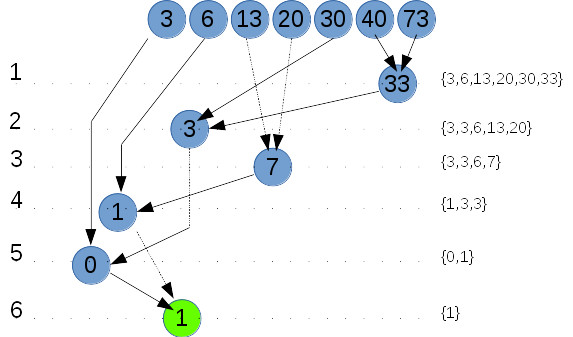
\includegraphics[width=\linewidth]
    {Biblio_PCmax_Rendu_exLDM_1_2m.jpg}
    \caption{Différentiation}
  	\end{subfigure}
\hfill% sinon, en fin de page, et pas sur la même ligne
% Backtracking à droite
	\begin{subfigure}[b]{0.45\linewidth}
    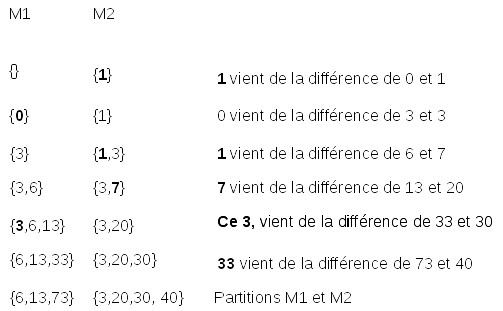
\includegraphics[width=\linewidth]
    {Biblio_PCmax_Rendu_exLDM_2_2m.jpg}
    \caption{Partitionnement (retour sur trace)}
  	\end{subfigure}
%CAPTION/FIGURE
  	\caption{LDM, avec $m=2$.}
  	\label{fig:LDM2M}
\end{figure}

\begin{example}
Soit $P=\{3,6,13,20,30,40,73\}$ l'ensemble des $p_j$.

40 et 73 sont les nombres les plus grands.
On les remplace dans $P$ par $73 - 40 = 33$, pour donner
$P=\{3,6,13,20,30,33\}$ et ainsi de suite.
La valeur restante est $P= \{1\}$, ce qui est le résultat de
l'opération.
Par un retour sur trace, nous obtenons le partitionnement suivant:
$m_1 = \{ 6,13,73 \}$ et $m_2 = \{ 3,20,30,40 \}$ (figure
\ref{fig:LDM2M}).

\end{example}

\bigskip

\item cas de $m>2$, $m$ sous-ensembles $m_1,m_2, \ldots, m_m $.

LDM effectue tout d'abord, une opération de préparation de
  l'instance du problème.
  Chaque élément de $P = \{ p_1, p_2, \ldots, p_n \}$ est converti en
  $m$-tuple.
  Les $m-1$ premiers composants sont vides, et le dernier (position $m$)
  est égal au nombre lui-même.
  Ainsi chaque
  $\underline{p_j} = \{p_{j 1}=0,p_{j 2}=0, \ldots, p_{j m}=\{p_j\}
  \}$

Puis, $n-1$ itérations des opérations suivantes sont effectuées:

\begin{itemize}
\item Soit $d(\underline{p_j})$ la différence entre la valeur maximale et la
valeur minimale des composants du sous-ensemble $\underline{p_j}$.
\item Extraction de $\underline{p_a}$ et $\underline{p_b}$ les deux m-tuples
qui ont la plus grande différence $d(\underline{p_a})$ et
$d(\underline{p_b})$.
Ces deux solutions partielles, sont combinées pour former une nouvelle
solution partielle $\underline{p_{ab}}$, en joignant le premier plus
petit élément (ou l'élément vide) de $\underline{p_a}$ avec le premier
élément le plus grand de $\underline{p_b}$, puis le deuxième élément
le plus petit de $\underline{p_a}$ avec le deuxième élément le plus
grand de $\underline{p_b}$ et ainsi de suite\ldots la nouvelle
solution partielle $\underline{p_{ab}}$, remplace $\underline{p_a}$ et
$\underline{p_b}$ dans l'instance.
\end{itemize}

Le résultat du partitionnement est donné après $n-1$ itérations.

%exemple
% ---------------------
\begin{example}

Soit $P=\{1,3,3,4,4,5,5,5\}$ avec un nombre de machines $m=3$.

\textbf{Création des $m$-tuples}:
\begin{multicols}{3}
$\underline{p_{1}} = \{,,1\}$\\
$\underline{p_{2}} = \{,,3\}$\\
$\underline{p_{3}} = \{,,3\}$\\
$\underline{p_{4}} = \{,,4\}$\\
$\underline{p_{5}} = \{,,4\}$\\
$\underline{p_{6}} = \{,,5\}$\\
$\underline{p_{7}} = \{,,5\}$\\
$\underline{p_{8}} = \{,,5\}$
\end{multicols}

\textbf{Itération 1}:\\
Les tuples qui ont la différence la plus grande sont
$\underline{p_{8}}$  et $\underline{p_{7}}$.
On combine $\underline{p_{8}}$ et $\underline{p_{7}}$ pour créer un
$\underline{p_{78}}$. Le premier plus petit élément de
$\underline{p_{8}}$ (élément vide) est joint par le premier plus grand
élément de $\underline{p_{8}}$ (5) pour donner $\underline{p_{78}} =
\{,5,5\}$. $d(\underline{p_{78}}) = 5-0 = 5$.
La nouvelle instance devient:
\begin{multicols}{3}
$\underline{p_{1}} = \{,,1\}$\\
$\underline{p_{2}} = \{,,3\}$\\
$\underline{p_{3}} = \{,,3\}$\\
$\underline{p_{4}} = \{,,4\}$\\
$\underline{p_{5}} = \{,,4\}$\\
$\underline{p_{6}} = \{,,5\}$\\
$\underline{p_{78}} = \{,5,5\}$\\
$d(\underline{p_{78}})=5$
\end{multicols}

\textbf{Itération 2}:\\
On conbine $\underline{p_{6}}$ avec $\underline{p_{78}}$ pour donner
$\underline{p_{678}} = \{5,5,5\}$. $d(\underline{p_{678}}) = 5-5 =
0$.
La nouvelle instance devient:
\begin{multicols}{3}
$\underline{p_{1}} = \{,,1\}$\\
$\underline{p_{2}} = \{,,3\}$\\
$\underline{p_{3}} = \{,,3\}$\\
$\underline{p_{4}} = \{,,4\}$\\
$\underline{p_{5}} = \{,,4\}$\\
$\underline{p_{678}} = \{5,5,5\}$\\
$d(\underline{p_{678}}) = 0$
\end{multicols}

\textbf{Itération 3}:\\
Les tuples qui ont la différence la plus grande sont
$\underline{p_{5}}$  et $\underline{p_{4}}$.
On les combine pour créer un $\underline{p_{45}}$. Le premier plus
petit élément de $\underline{p_{5}}$ (élément vide) est joint par le
premier plus grand élément de $\underline{p_{4}}$ (4) pour donner
$\underline{p_{45}} = \{,4,4\}$. $d(\underline{p_{45}}) = 4-0 = 4$.
La nouvelle instance devient:
\begin{multicols}{3}
$\underline{p_{1}} = \{,,1\}$\\
$\underline{p_{2}} = \{,,3\}$\\
$\underline{p_{3}} = \{,,3\}$\\
$\underline{p_{45}} = \{,4,4\}$\\
$\underline{p_{678}} = \{5,5,5\}$\\
$d(\underline{p_{45}}) = 4$
\end{multicols}

\textbf{Itération 4}:\\
Les tuples qui ont la différence la plus grande sont
$\underline{p_{45}}$  et $\underline{p_{3}}$.
On les combine pour créer un $\underline{p_{345}}$. Le premier plus
petit élément de $\underline{p_{45}}$ (élément vide) est joint par le
premier plus grand élément de $\underline{p_{3}}$ (3) pour donner
$\underline{p_{345}} = \{3,4,4\}$. $d(\underline{p_{345}}) = 4-3 =
1$.
La nouvelle instance devient:
\begin{multicols}{3}
$\underline{p_{1}} = \{,,1\}$\\
$\underline{p_{2}} = \{,,3\}$\\
$\underline{p_{345}} = \{3,4,4\}=1$\\
$d(\underline{p_{345}}) = 1$
\end{multicols}

\textbf{Itération 5}:\\
Les tuples qui ont la différence la plus grande sont
$\underline{p_{345}}$  et $\underline{p_{2}}$.
On les combine pour créer un $\underline{p_{2345}}$. Le premier plus
petit élément de $\underline{p_{345}}$ (3) est joint par le premier
plus grand élément de $\underline{p_{2}}$ (3) pour donner
$\underline{p_{2345}} = \{(3,3),4,4\}$. La première association, vient
d'être créée. elle a pour valeur 6.
$d(\underline{p_{2345}}) = (3+3)-4 = 6-4=2$. La nouvelle instance devient:
\begin{multicols}{2}
$\underline{p_{1}} = \{,,1\}$\\
$\underline{p_{2345}} = \{(3,3),4,4\}$\\
$\underline{p_{678}} = \{5,5,5\}$\\
$d(\underline{p_{2345}}) = 2$
\end{multicols}

\textbf{Itération 6}:\\
Les tuples qui ont la différence la plus grande sont
$\underline{p_{2345}}$  et $\underline{p_{1}}$.
On les combine pour créer un $\underline{p_{2345}}$. Le premier plus
petit élément de $\underline{p_{2345}}$ (4) est joint par le premier
plus grand élément de $\underline{p_{2}}$ (1) pour donner
$\underline{p_{12345}} = \{(3,3),(1,4),4\}$. $d(\underline{p_{12345}})
= (3+3)-4 = 6-4=2$.
La nouvelle instance devient:
\begin{multicols}{2}
$\underline{p_{12345}} = \{(3,3),(1,4),4\}=2$\\
$\underline{p_{678}} = \{5,5,5\}$\\
$d(\underline{p_{12345}}) = 2$
\end{multicols}

\textbf{Itération 6}:\\
Reste à combiner $\underline{p_{12345}}$ et $\underline{p_{678}}$.
Le premier plus petit élément de $\underline{p_{12345}}$ (4) est joint
avec le premier plus grand de $\underline{p_{678}}$ (5) et ainsi de
suite\ldots pour créer le résultat final
$\underline{P_{LDM}}= \{(3,3,5),(1,4,5),(4,5)\}$.\\

Nous avons donc un makespan $C_m^{LDM}(P) = 11$ alors que
$C_m^{\star}(P) = 10$ avec $\underline{P^{\star}}=
\{(5,5),(1,4,5),(4,3,3)\}$.
\end{example}

\end{itemize}


% Complexité
% -------------------------------------------------------
\begin{theoreme}
\begin{flushleft}
\begin{tabular}{|p{8cm}p{6cm}|}
% TITRES (pas de titre)
\hline
% Ligne blanche
& \\
% Ligne Complexité
Complexité en temps \cite{michiels2003performance}:& $O(n \cdot \log n) $
\\	% pas de ligne \hline
% Ligne blanche
& \\
% RATIO
Ratio \cite{michiels2003performance} &\\
% RATIO M= 2
pour $m=2$  & $\Gamma(LDM) = \frac{7}{6}$\\
pour $m\geq 3$ & $ \frac{4}{3}-\frac{1}{3 \cdot (m-1)} \leq
   					\Gamma(LDM) \leq
   					\frac{4}{3}-\frac{1}{3 \cdot m}$
\\
% Ligne blanche
& \\
\hline
\end{tabular}
%pas de legende
\end{flushleft}
\end{theoreme}


\subsubsection{Autres algorithmes}

D'autres algorithmes basés sur le partitionnement de nombres:

\begin{itemize}
\item MPS, de Paletta \emph{et al.} \cite{paletta2007new}
\item SPS, de Chiaselotti \emph{et al.} \cite{chiaselotti2010minimizing}
\end{itemize}

\section{Synthèse} \label{sec:synthese}


\subsection{Comparaisons} \label{ssec:syntheseComparaison}

Chaque étude du problème \problemGrahamP tente
d'améliorer le ratio d'approximation, ainsi que le coût en temps requis
pour obtenir cette solution approchée,
soit en reprenant une piste déjà explorée afin de l'optimiser,
soit en expérimentant d'autres méthodes.
Les résultats théoriques, définis et déterminés par démonstrations ne sont que des indications ``au pire cas''. Les performances réelles sont en moyennes meilleures. 


\subsubsection{Théoriques}

% -------------------------------------------------------
% Tableau coupé en 2 car trop large !
% -------------------------------------------------------
% TABLEAU Comparatif RATIOS COÛTS EN TEMPS de chaque approche
% quand on les a !
% diagbox permet d'avoir une barre oblique pour les deux entrées
% \backslashbox{Instructions}{Donnée} & Simple & Multiple NE FONCTIONNE PAS
% on cadre à gauche le tableau pour avoir plus de place
% -------------------------------------------------------
Le tableau~\ref{table:synth} est un comparatif des performances
calculées et déterminées de chaque algorithme présenté.

% 1/2
\begin{table}
\begin{center}
\begin{tabular}{p{0.17\linewidth}
				p{0.16\linewidth}
				p{0.16\linewidth}
				p{0.16\linewidth}
				p{0.16\linewidth}
				p{0.16\linewidth}}

% ----------------------------------------------------
% TITRES
% ----------------------------------------------------
\toprule
performance 						&
							LPT 	&
							LPT-Rev &
							Slack 	&
							multifit&
							combine
%							listfit &
%							PA		&
%							PTAS	&
%							LDM  	\\
\\
\midrule

% --------------------------
% LIGNE O()
% --------------------------
Complexité \newline (en temps) 		&
							$O(n \cdot \log n) $ (*) &		% LPT
							$O(n \cdot \log n)$  (*) & 		% LPT-REV
							$O(n \cdot \log n)$  (*) & 		% SLACK
							$O(n \log n + kn \log m)$& 		% MULTIFIT
							$O(n \log n + kn \log m)$		% COMBINE

\\
% --------------------------
% LIGNE Ration
% --------------------------
Ratio \newline (pire des cas)		&
							$\frac{4}{3} - \frac{1}{3m}$&		% LPT
							$\frac{4}{3} - \frac{1}{3(m-1)}$&	% LPT-REV
							-&								% SLACK (pas d'info)
							$1,220 + 2^{-k}$& 					% MULTIFIT
							$\frac{13}{12} + 2^{-k}$			% COMBINE
%---------------------------
\\
\bottomrule
\end{tabular}
\end{center}

% 2/2
\begin{center}
\begin{tabular}{p{0.17\linewidth}
				p{0.16\linewidth}
				p{0.16\linewidth}
				p{0.16\linewidth}
				p{0.25\linewidth}}


% ----------------------------------------------------
% TITRES
% ----------------------------------------------------
\toprule
performance 						&
							listfit &
							PA		&
							PTAS	&
							LDM
\\
\midrule

% --------------------------
% LIGNE O()
% --------------------------
Complexité \newline (en temps) &
							$O(n^2 \log(n) + k \cdot n^2 \log(m))$&	% LISTFIT
							-& 						% PA (pas d'infos)
							$ O(( \frac{n}{\epsilon})^\frac{1}{\epsilon ^ 2})$&
					 		$O(n \cdot \log n) $	% LDM

\\
% --------------------------
% LIGNE Ration
% --------------------------
Ratio \newline (pire des cas)		&
							$\frac{13}{12} + 2^{-k}$&		% LISTFIT
							-&								% PA (pas d'info)
							$1 + \epsilon$	&				%PTAS
							compris entre \newline						% LDM
								$\frac{4}{3}-\frac{1}{3 \cdot m}$ et	% LDM
								\newline 								% LDM
								$\frac{4}{3}-\frac{1}{3 \cdot (m-1}$	%LDM

%---------------------------
\\
\bottomrule
\end{tabular}
\end{center}
\caption{\label{table:synth}
Comparaison des performances des algorithmes présentés.
$n$ est le nombre de jobs à planifier.
$m$ est le nombre de machines parallèles identiques.
$k$ est un nombre d'itérations, soit  fixé via un paramètre de l'algorithme, ou le résultat d'une condition d'arrêt.
$\epsilon$ est un nombre positif (e.g.\ $\frac{1}{5}$) et désigne le ratio d'approximation d'un PTAS.
(*) signifie qu'il faut rajouter $(n \cdot \log m)$ si on prend en compte le tri des jobs au
préalable.
}
\end{table}

LPT rule et LPT-REV présentent un ratio d'approximation qui s'approche
du pire cas lorsque le nombre de machines augmente.
Multifit, Combine et Listfit se suivent dans leurs performances
(ListFit est plus coûteux en temps).
Concernant le PTAS, plus $\epsilon$ est petit (ratio tend vers $1$)
plus l'algorithme se rapproche de la solution optimale, mais plus il
pèse dans la complexité en temps (exponentiel en $\epsilon$).


\subsubsection{Expérimentales}

\begin{figure}
\centering
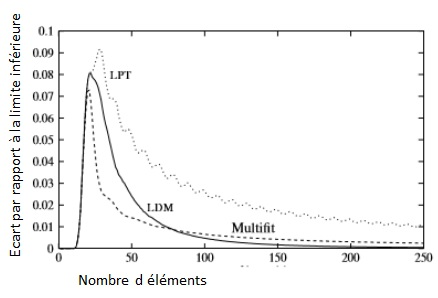
\includegraphics[width=10cm,height=6.80cm]
{Biblio_PCmax_Rendu_CompborneInf_LPT_LDM_MULTIFIT.jpg}
\caption{Écarts moyen de LPT, LDM et Multifit par rapport à la borne
  inférieure de 10\,000 instances créées pour chaque nombre $n$
  d'éléments et $m=10$ machines~\cite{michiels2003performance}.}
\label{comparaison:LPTLDMMFBorneInf}
\end{figure}

En général, LPT donne des performances pratiques bien meilleures que
les ratios théoriques attendus \cite{della2018longest}, surtout dans
les instances à nombre élevé de jobs.

Michiels \emph{et al.}
\cite{michiels2003performance} étudient les performances des trois
algorithmes phares (LPT, LDM, et Multifits), pour un nombre m=10
machines, et en fonction du nombre $n$ d'éléments.
Pour chaque n, 10 000 instances sont créées, à l'aide de nombres
(temps des jobs) uniformément répartis (instances uniformes) dans
l'intervalle [0,1].
La figure \ref{comparaison:LPTLDMMFBorneInf} représente l'écart moyen
de chaque algorithme par rapport à la borne inférieure (théorème
\ref{borneMini}).
LPT est le moins performant, et Multifit supplante LDM à partir de
$n=79$ éléments.
Néanmoins, cette étude se base sur des éléments uniformément répartis,
condition où LDM est très performant.

Slack (algorithme~\ref{algo:SLACK}), qui est une heuristique basée sur LPT 
accompagné d'une recherche locale devient globalement plus performant 
que LDM \cite{della2018longest}.

Gupta \emph{et al.}\ prouvent que les performances de ListFit (algorithme~\ref{algo:LISTFIT}) sont
supérieures à LPT, Multifit et Combine. Ceux-ci sont comparés
\cite{gupta2001listfit,lee1988multiprocessor} suivant des
indices, en mettant de côté le nombre $k$ nécessaires à l'achèvement des
algorithmes.
Behera \emph{et al.}~\cite{behera2012comparison} comparent dans une étude le
coût processeur 
(table~\ref{table:comparaisonTempsMultifitCombineListfitBehera}) 
de chaque heuristique, ce qui indique que Listfit est très gourmand.


\begin{table}
\begin{center}
\begin{tabular}{p{0.19\linewidth}
				p{0.19\linewidth}
				p{0.19\linewidth}
				p{0.19\linewidth}
				p{0.19\linewidth}}
% ----------------------------------------------------
% TITRES
% ----------------------------------------------------
\toprule
$n$		&	$m$	&	Multifit	&	Combine	&	Listfit
\\
\midrule
% --------------------------
% LIGNE des 100
% --------------------------
100		&	2	&	20			&	22		&	1767 	\\
		&	3	&	24			&	32		&	1968	\\
		&	6	&	20			&	44		&	3293	\\
		&	8	&	20			&	56		&	3755
\\
200		&	2	&	44			&	66		&	7269 	\\
		&	3	&	44			&	66		&	8153	\\
		&	6	&	64			&	132		&	13695	\\
		&	8	&	64			&	154		&	15422
\\
300		&	2	&	88			&	120		&	15663	\\
		&	3	&	112			&	132		&	17671	\\
		&	6	&	108			&	176		&	25673	\\
		&	8	&	132			&	198		&	29558
% FIN ----------------------------------------
\\
\bottomrule
\end{tabular}
\end{center}
\caption{\label{tab:XP} Comparaison \cite{behera2012comparison} des temps moyens pour Multifit,
  Combine et Listfit (en $10^{-6}$ secondes).}
\label{table:comparaisonTempsMultifitCombineListfitBehera}  
\end{table}


\subsection{De la recherche d'informations}
\label{ssec:syntheseRechercheInformation}

Il a été très difficile, voire impossible de trouver plus
d'informations sur les performances de PA (algorithme~\ref{algo:PA}, résolution du
problème \problemGrahamP par programmation linéaire), du PTAS
dual-approximation (algorithmes~\ref{algo:PTASDual1_5} et \ref{algo:PTASDual1_6}).
En effet, il aurait été intéressant d'avoir un aperçut de la
complexité en temps de PA (Programmation linéaire + Branch\&Bound) et
l'algorithme générique (non optimisé pour $\epsilon = \frac{1}{5}$ et
$\epsilon = \frac{1}{6}$) du PTAS dual-approximation en programmation
dynamique.

\section{Conclusion} \label{sec:conclusion}

Dans cette bibliographie non-exhaustive, nous venons de voir
différentes approches qui tentent de répondre au problème
d'ordonnancement \problemGrahamP, soit directement, soit indirectement
via des problèmes similaires, tels que le Bin-Packing ou le
partitionnement de nombres.
Chacune de ces méthodes a ses avantages et ses défauts.
Soit leur complexité en temps est intéressante, mais leur ratio
d'approximation est élevé, ou inversement, le résultat obtenu est très
proche de l'optimal, au détriment d'un coût élevé en temps.

Il sera intéressant de définir un protocole expérimental afin de créer
un spectre d'instances du problème plus complet, pour produire
une comparaison d'un ensemble d'heuristiques.

Et enfin, ces résultats pourrons être utilisés pour d'autres problèmes
d'ordonnancements (contraintes, processeurs/machines hétérogènes).

\section{Remerciements} \label{sec:remerciements}

J'adresse mes remerciements aux personnes qui m'ont aidé dans la réalisation de ce document. 
Laurent Philippe, professeur à l'université de Franche-Comté, 
Louis-Claude Canon, maître de conférence, et 
Julien Bernard, maître de conférence. 
Il m'ont tous guidé dans mon travail, en trouvant des solutions pour avancer, 
et en me fournissant d'importantes informations concernant 
le problème \problemGrahamP et les travaux qui s'y rapportent. 
Je les remercie, également, pour leur disponibilité, 
et le temps qu'ils m'ont consacré, pour répondre à mes questions, 
et leur retours critiques. 

Et merci aussi, à Anne-Sophie, pour son aide à la relecture et à la correction de ce document.


\medskip


\bibliographystyle{plain}				% NE PAS ENLEVER !!!!!!!!!!
\bibliography{Bibliographie}			% Utilise Bibliographie.bib








\end{document}
